\glsresetall

% Don't show subsections in the TOC.
\addtocontents{toc}{\protect\setcounter{tocdepth}{1}}


This chapter presents the results of the fuel cell model.  The first section investigates the operation of the cell during a baseline polarization test.  The next six sections vary certain properties, such as temperature and pressure, and observe the effects on the polarization curve.  Then, Sections~\ref{sec:SimpleCell} and~\ref{sec:SegCell} show variations of the cell model, specifically a simplified model and a model with multiple segments down the length of the channel.  The final section (\ref{sec:Cycle}) shows the dynamics of the model under a cyclical load.  All of the results are from the fuel cell model except for the experimental data used in Figures~\ref{fig:BaselinePolarization} and \ref{fig:TemperaturePolarization} through \ref{fig:CaHumidityPolarization} to benchmark the model.


\section{Baseline Polarization Test}
\label{sec:Baseline}

\subsection{Test Conditions}
\label{sec:Baseline-Conditions}

The \modelica{TestStand} model presented in \autoref{sec:TestStand} applies boundary conditions to the \modelica{Cell} model.  Under the baseline conditions, the temperature of the reactant supplies and the exterior x-axis boundary of the flow plates is \SI{60}{\celsius}.  This temperature is used to initialize the layers as well.  Both outlets are maintained at \SI{48.3}{kPag}.  The cell operates on \s{H2} humidified to 80\% and air humidified to 50\%.  The reactant supply varies stoichiometrically according to the electrical load.  The stoichiometric ratio is 1.5 in the anode and 2.0 in the cathode.  After an initial three minutes to reach steady conditions at \SI{0.1}{mA}, the electrical load is ramped at a rate of \SI{0.3}{A/cm^2} per hour for ten hours or until the cathode is depleted of \s{O2}.  A slow ramp rate is used so that the dynamic effects are negligible.  Although the model has options to assume steady state conditions, the states are generally necessary to avoid nonlinear systems of equations.

The area of the cell is \SI{50}{cm^2}.  There is one subregion for each layer.  Ideal gases are assumed.  Liquid is included.  The double layer capacitances are not included in order to eliminate some of the dynamics.  The key physical parameters of the model are listed in \autoref{tab:CellParams}.  The values roughly correspond to a test cell used at the \n{HNEI} to provide the benchmark data, which is shown in the results.  Where possible, the values are cited and justified in the model documentation (\autoref{chap:Doc}).  Due to the complexity of the model and the limitations of physical sensors, it is not possible to directly establish some of the parameters, especially those that deal with transfer rates.  This is a known issue with fuel cell models in general~\cite{Faghri2005}.  

Other parameters are listed in the tables of \autoref{chap:Doc}.  The thermodynamic correlations from McBride et al.~\cite{McBride2002} are used for the fluids.  The fluidity and thermal resistivities are based on the correlations from Svehla et al.~\cite{Svehla1995} and tables from Incropera and DeWitt~\cite{Incropera2002}.  The kinetic theory of gases~\cite{Present1958} is used to approximate properties that are not available directly.  

%The geometries of the cell's flow plates were established by General Motors with serpentine flow fields of two parallel anode channels and three parallel cathode channels.  The \n{MEA} was produced by Ion Power~\cite{IonPower2009} and the \np{GDL} are model 25BC from SGL~\cite{SGL2004}.  The cell was operated under stoichiometrically varying reactant flows on a test stand from Greenlight Innovation at the \n{HNEI}.  

\begin{sidewaystable}[hbtp]
  \caption{Key parameters of the fuel cell model}
  \label{tab:CellParams}
  \begin{tabular}{llllllll}
    \toprule
     & \textbf{anFP} & \textbf{anGDL} & \textbf{anCL} & \textbf{PEM} & \textbf{caCL} & \textbf{caGDL} & \textbf{caFP} \\
    \midrule
    Volumetric porosity & 0.059 & 0.8 & 0.4 & --- & 0.4 & 0.8 & 0.042 \\
    Thickness / mm & 10 & 0.235 & 0.029 & 0.04 & 0.029 & 0.235 & 10 \\
    Channel length / m & 1.62 & --- & --- & --- & --- & --- & 1.06 \\
    Hydraulic diameter / \SI{}{mm^2} & 0.94 & --- & --- & --- & --- & --- & 0.82 \\
    Electronic conductivity / \SI{}{S.cm^{-1}} & 680 & 3.3\footnote{\label{note1}This is for the bulk media (i.e., after accounting for porosity).} & 3.3\footnoteref{note1} & --- & 3.3\footnoteref{note1} & 3.3\footnoteref{note1} & 680 \\
    Protonic conductivity\footnote{This only describes coupling with the solid.  Electro-osmotic drag (coupling with \s{H2O}) introduces additional resistance.} / \SI{}{S.cm^{-1}} & --- & --- & 0.1 & 0.1 & 0.1 & --- & --- \\
    Thermal resistivity of carbon / \SI{}{m.K.W^{-1}} & 0.01 & 0.85\footnoteref{note1} & 0.85\footnoteref{note1} & --- & 0.85\footnoteref{note1} & 0.85\footnoteref{note1} & 0.01 \\
    Thermal resistivity of dry ionomer / \SI{}{m.K.W^{-1}} & --- & --- & 6.25 & 6.25 & 6.25 & --- & --- \\
    Exchange current density @ \SI{300}{K} / \SI{}{A.cm^{-2}} & --- & --- & 1 & --- & \num{2.3E-5} & --- & --- \\
    Activation energy / V & --- & --- & 0 & --- & 0.75 & --- & --- \\
    Contact angle & \SI{90}{\degree} & \SI{140}{\degree} & \SI{140}{\degree} & --- & \SI{140}{\degree} & \SI{140}{\degree} & \SI{90}{\degree} \\
    Effective pore radius / \SI{}{\micro.m} & --- & 32 & 5 & --- & 5 & 32 & --- \\
    Evaporation interval / ms & 16 & 16 & 16 & --- & 16 & 16 & 16 \\
    Absorption interval / s & --- & --- & 33 & --- & 33 & --- & --- \\
    Common mobility factor & \num{E7}\footnote{\label{note2}This is in the x direction (through the cell).  In the y direction (down the channel), it is infinite.} & 1.7 & 1.7 & $\infty$ & 1.7 & 1.7 & \num{E7}\footnoteref{note2} \\
    Mobility factor between gas and liquid & \num{E6}\footnoteref{note2} & $\infty$ & $\infty$ & --- & $\infty$ & $\infty$ & \num{E6}\footnoteref{note2} \\
    Mobility factor between \s{H+} and \s{H2O} & --- & --- & 0.02 & 0.02 & 0.02 & --- & --- \\
    Mobility factor between \s{H2O} and \s{SO3-} & --- & --- & 1 & 1 & 1 & --- & --- \\
    Common thermal independence factor & \num{E5} & 0 & 0 & 0 & 0 & 0 & \num{E5} \\
    \bottomrule
  \end{tabular}
\end{sidewaystable}


\subsection{Results and Discussion}
\label{sec:Baseline-Results}

\begin{contextbox}
  Modeling and simulation statistics:
  \begin{itemize}
    \item Number of variables: 6887
    \item Number of time-varying variables: 2749
    \item Number of states: 55
    \item Sizes of the nonlinear systems of equations: None
    \item Sizes of the linear systems of equations: 1 set of 9, 1 set of 8, 1 set of 6, 2 sets of 5, 9 sets of 4, 18 sets of 3, 97 sets of 2
    \item Translation time: \SI{23}{s}
    \item Simulation time: \SI{1.56}{s}
  \end{itemize}
\end{contextbox}

The cell model is much more complex than the models of \autoref{chap:Basic}, but as indicated by the simulation time of under two seconds, the translator and solver handle it well.  There are no nonlinear systems of equations.  The 55 states of the model include the following temperatures:
\begin{enumerate*}
  \item anFP gas
  \item anFP liquid
  \item anFP solid (graphite)
  \item anGDL (all phases combined)
  \item anCL (all phases combined)
  \item PEM
  \item caCL (all phases combined)
  \item anGDL (all phases combined)
  \item caFP gas
  \item caFP liquid
  \item caFP solid (graphite)
\end{enumerate*}
It is assumed that all of the species have the same temperature in the interior layers, regardless of phase, because the associated time constants were calculated by the model to be very quick (between \num{E-11} and \SI{E-7}{s}).  The following 24 amounts of material also appear as states:
\begin{enumerate*}
  \item \s{H2} in the anFP, anGDL, and anCL (3)
  \item \s{H2O} as gas in the anFP, anGDL, anCL, caCL, caGDL, and caFP (6)
  \item \s{H2O} as liquid in the anFP, anGDL, anCL, caCL, caGDL, and caFP (6)
  \item \s{H2O} in the ionomer of the anCL, PEM, and caCL (3)
  \item \s{N2} in the caCL, caGDL, and caFP (3)
  \item \s{O2} in the caCL, caGDL, and caFP (3)
\end{enumerate*}
There are 14 states related to velocity:
\begin{enumerate*}
  \item x-direction velocity of \s{H2} in the anGDL and anCL (2)
  \item x-direction velocity of \s{H2O} gas in the anGDL, caCL, and caGDL (3)
  \item x-direction velocity of \s{H2O} liquid in the anGDL, anCL, caCL, and caGDL (4)
  \item y-direction velocity of \s{H2O} liquid in the anFP and caFP (2)
  \item x-direction velocity of \s{H2O} in the ionomer of the anCL and caCL (2)
  \item x-direction velocity of \s{N2} in the caGDL (1)
\end{enumerate*}
The y-direction velocities are constrained by the boundary conditions, so they are not independent for each species.  The final group of states contains these currents:
\begin{enumerate*}
  \item x- and y-direction currents of \n{H2O} gas in the anFP (2)
  \item x-direction current of \n{O2} in the caCL and caGDL (2)
  \item x- and y-direction currents of \n{N2} in the caFP (2)
\end{enumerate*}
For numerical reasons, it is sometimes better to choose currents as states instead of velocities.

\autoref{fig:BaselinePolarization} compares the polarization of the cell model against seven runs of the experimental cell over the span of about a week.  There are significant differences.  At the lowest current measured by experiment (\SI{0.1}{A/cm^2}), the model overpredicts the voltage.  This may be due to the \n{H2} crossover current, which was significant in the experimental cell but not included in the model.  The modeling framework could be used to include this phenomena, but that development is left as future work.  At mid-range current, the model underpredicts the voltage.  This is a consequence of tuning the exchange current density to compromise between the low and mid-range current given the fact that \n{H2} crossover is not included.  At higher currents, the voltage of the experimental cell drops---probably due to the effect of liquid water on the concentration\slash{}transport losses.  Although liquid is included in the model and begins to fill the pores of the cathode \n{GDL} as will be shown, it does not have a significant effect on the polarization.

\begin{figure}[htbp]
  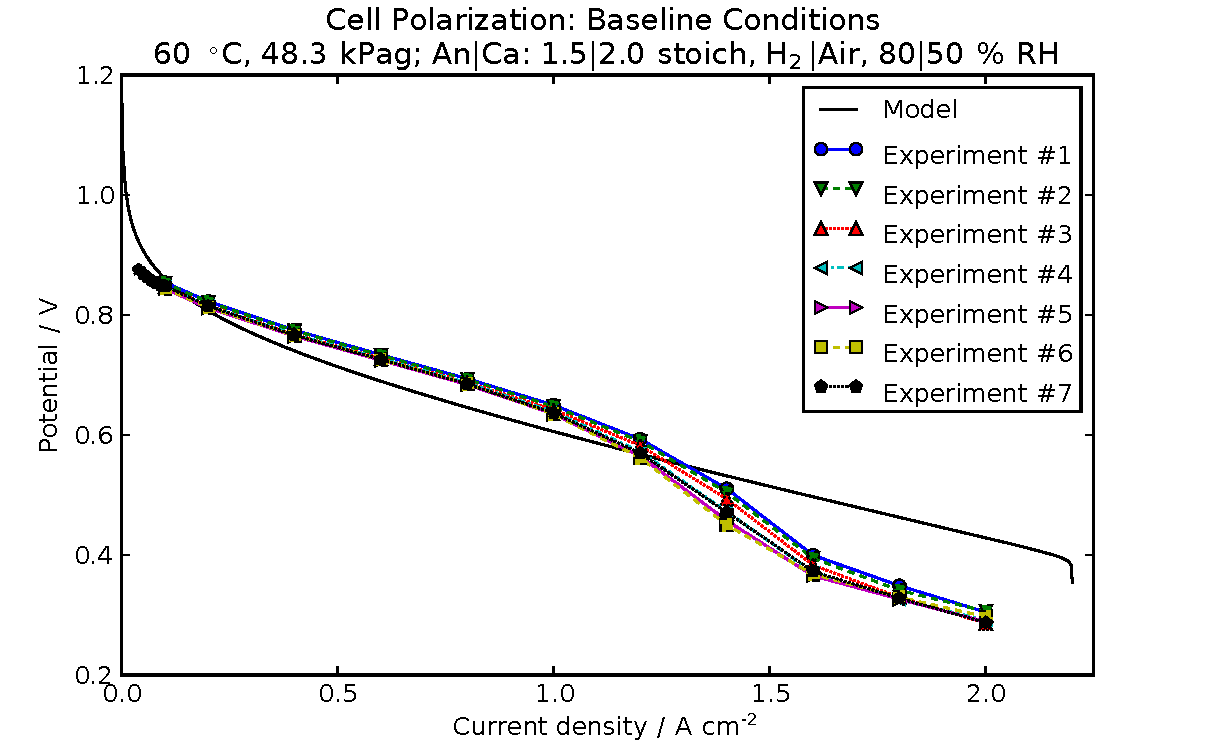
\includegraphics[width=\linewidth]{Results/Cell/Model/Baseline/Polarization}%
  \caption{Polarization curves of the cell for the baseline polarization}%
  \label{fig:BaselinePolarization}
\end{figure}

\autoref{fig:BaselineWater} contains a Sankey diagram of the energy balance on the cell at \SI{1.5}{A/cm^2}.  It should be noted that the Sankey diagram indicates the direction of transfer of the quantity (here, energy), not necessarily the direction of material transfer.  In \autoref{fig:BaselineWater}, the inlet and outlet of each stream is combined.  While this helps to show the net rate of contribution, it may be confusing in the case of water.  Since the enthalpy of formation of water is negative by convention, an inflow of water appears as an outflow of energy and vice versa.

The thermodynamic efficiency is only 36\% at this rather high current of \SI{1.5}{A/cm^2}.
% 38.6/(38.6 + 14.3 + 54.3) = 36%
The fact that the main trunk of the Sankey diagram has uniform  thickness indicates that there is no transient energy storage (and the model equations are consistent).  If the load is ramped quickly during a polarization test (e.g., in \autoref{sec:Cycle}), then the energy balance includes significant transients.  These would appear as a taper in the thickness of the trunk between the inputs and outputs.

\begin{figure}[htbp]
  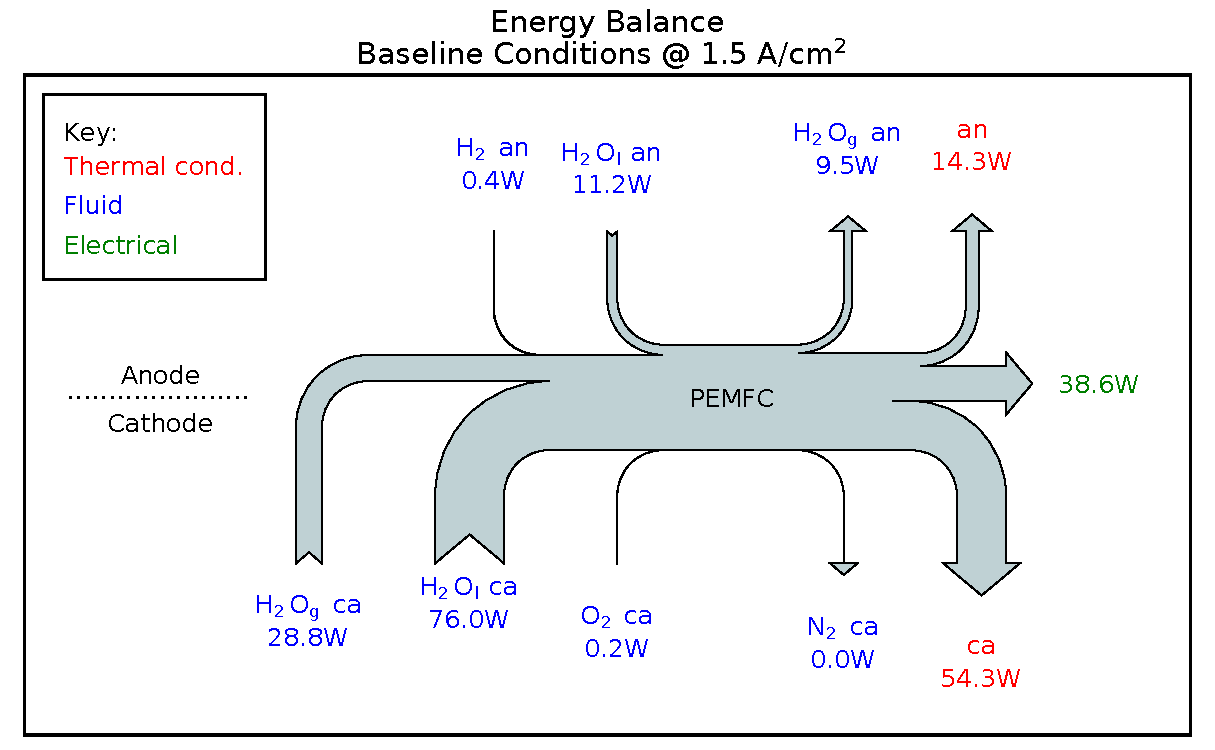
\includegraphics[width=\linewidth]{Results/Cell/Model/1/Energy}%
  \caption{Energy balance under the baseline conditions at \SI{1.5}{A/cm^2}}%
  \label{fig:BaselineEnergy}
\end{figure}

\autoref{fig:BaselineVoltages} shows the losses in the cell.  As expected, the cathode overpotential is dominate.  The next most significant loss is protonic conduction through the catalyst layers and the \n{PEM}.  The anode operates in the regime where the overpotential is linear, in contrast to the Tafel or logarithmic\slash{}exponential regime of the cathode.  The loss due to \n{O2} transport, while small in scale, does begin to increase exponentially near the limiting current density.

\begin{figure}[htbp]
  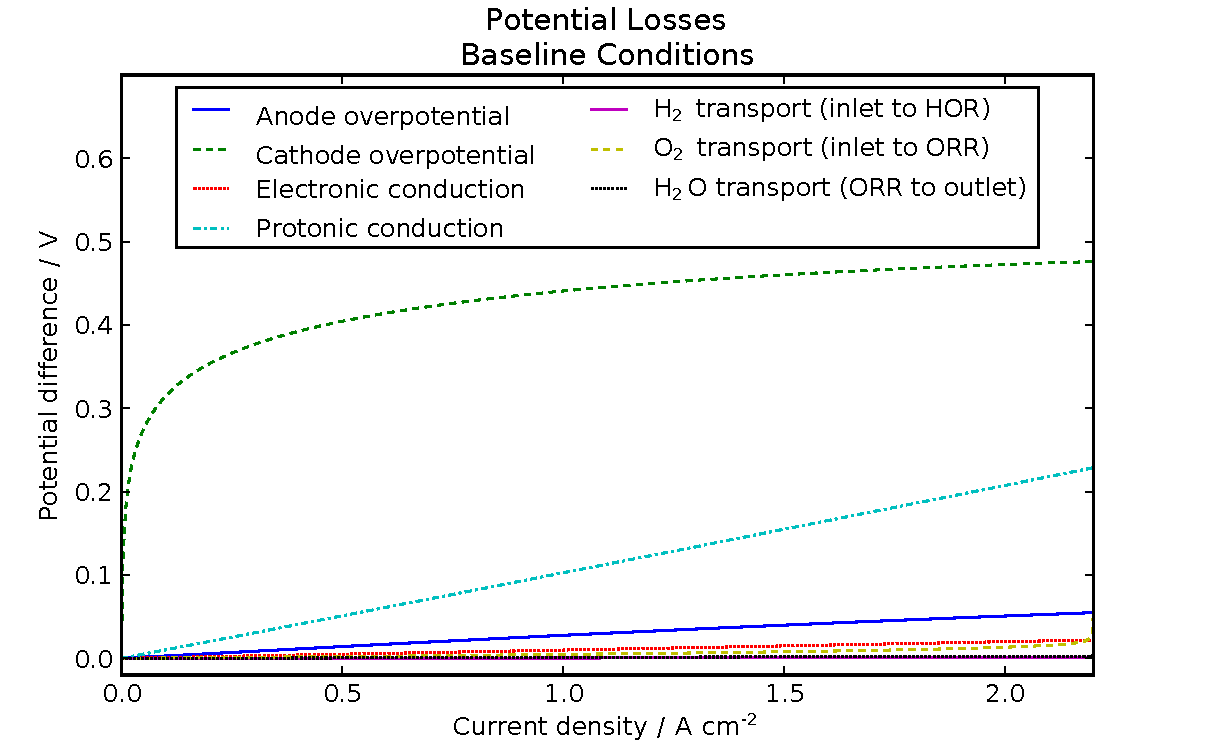
\includegraphics[width=\linewidth]{Results/Cell/Model/1/PotentialLosses}%
  \caption{Potential losses through the cell during the baseline polarization}%
  \label{fig:BaselineVoltages}
\end{figure}

\autoref{fig:BaselineElectricalLosses} gives information about location of the Ohmic losses, which were grouped as electronic and protonic in \autoref{fig:BaselineVoltages}.  The loss in the \n{PEM}, which is protonic, is the most significant.  The catalyst layers also have large losses, which are a combination of electronic and protonic.  The resistance in the \np{GDL} and flow plates is relatively small.

\begin{figure}[htbp]
  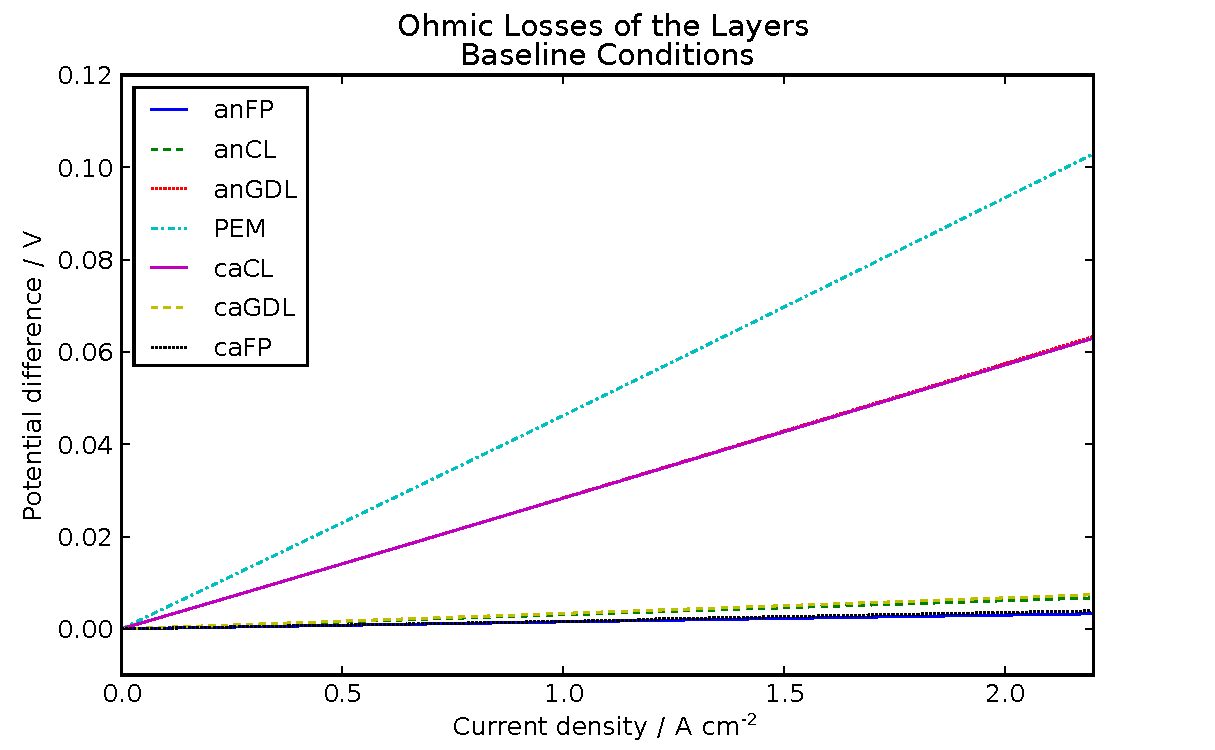
\includegraphics[width=\linewidth]{Results/Cell/Model/1/ElectricalLosses}%
  \caption{Electrical losses in the cell during the baseline polarization}%
  \label{fig:BaselineElectricalLosses}
\end{figure}

The losses generate heat and increase the temperature of the interior of the cell as shown in \autoref{fig:BaselineTemperature}.  The hottest region is the cathode catalyst layer due to the large activation overpotential.  The neighboring regions---the cathode \n{GDL} and the \n{PEM}---have the next highest temperatures.  The cathode is generally hotter than the anode.  More heat is rejected through the cathode flow plate, as was evident in \autoref{fig:BaselineEnergy}.

\begin{figure}[htbp]
  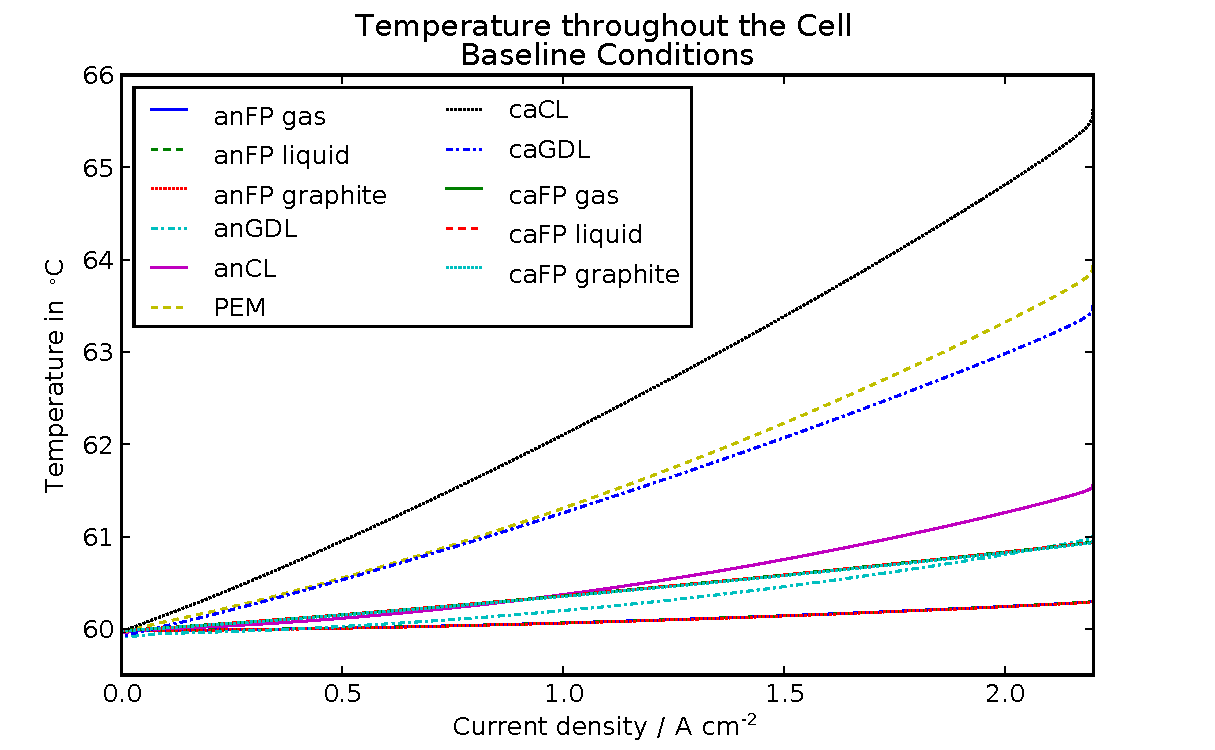
\includegraphics[width=\linewidth]{Results/Cell/Model/1/Temperature}%
  \caption{Temperatures through the cell during the baseline polarization}%
  \label{fig:BaselineTemperature}
\end{figure}

\autoref{fig:PressureGas} shows the pressure of the gas throughout the cell.  It is highest in the cathode flow plate, as this is required to transport \n{O2} into the cell.  Above \SI{2}{A/cm^2}, the pressure of the cathode gas begins to decrease as the concentration limit is reached.  The pressures of the anode are very close to the outlet pressure of \SI{48.3}{kPag}.   \autoref{fig:ChannelPressureDrop} shows the pressure loss along the channels.  The pressure difference between the cathode inlet and outlet is much greater (a factor of nearly 20) than the difference between the anode inlet and outlet.  This is due to the higher viscosity of air relative to \n{H2} and the higher velocity required to deliver \n{O2} since it is at lower concentration in the cathode than \n{H2} is in the anode.

\begin{figure}[htbp]
  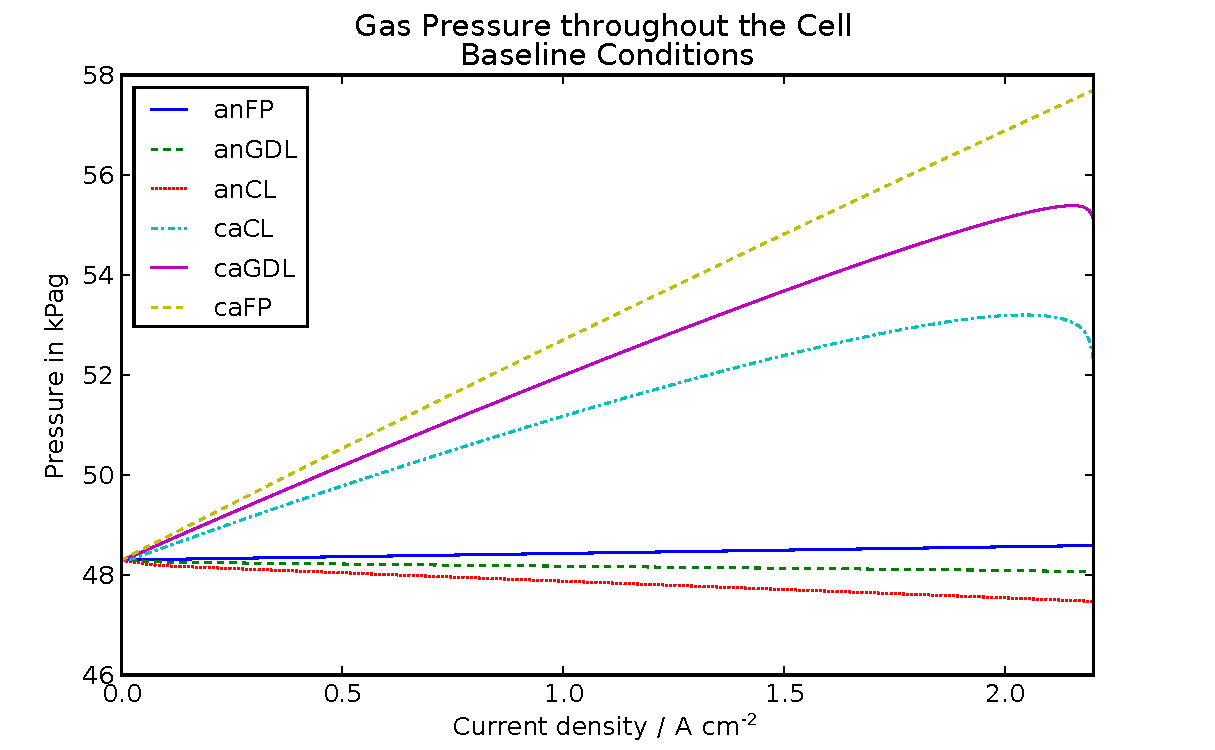
\includegraphics[width=\linewidth]{Results/Cell/Model/1/PressureGas}%
  \caption{Total pressure of the gas during the baseline polarization}%
  \label{fig:PressureGas}
\end{figure}

\begin{figure}[htbp]
  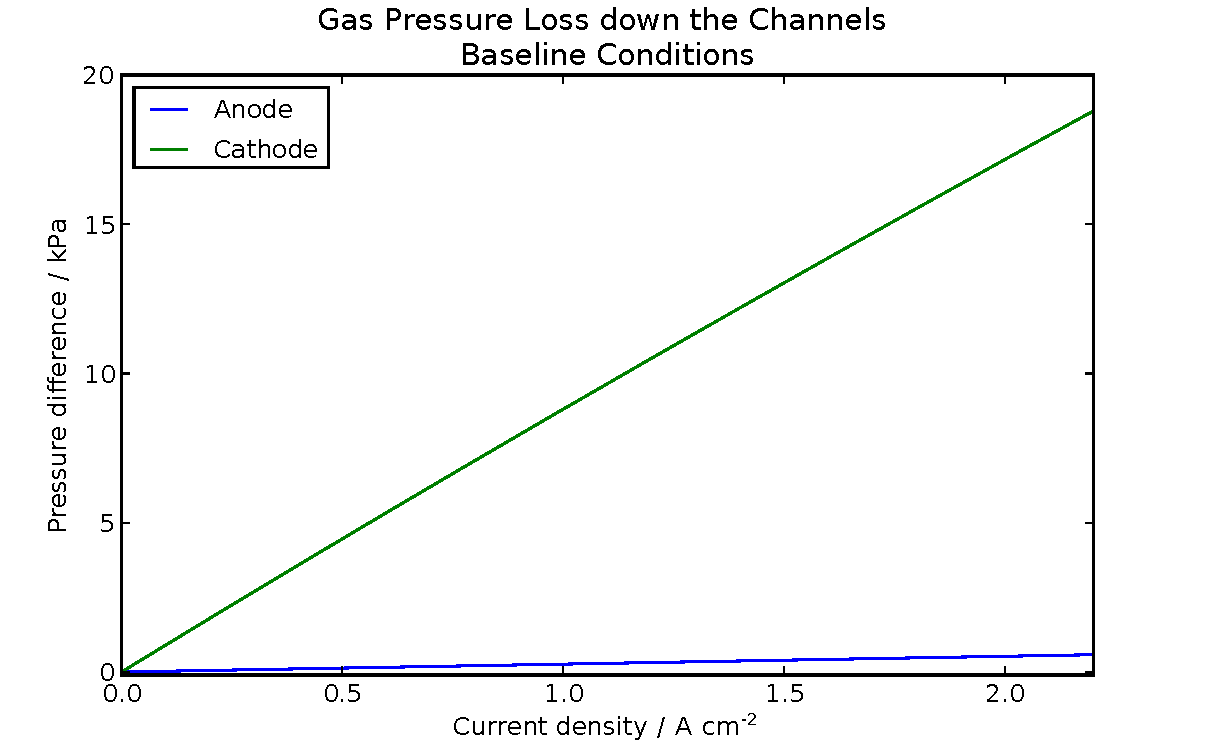
\includegraphics[width=\linewidth]{Results/Cell/Model/1/ChannelPressureDrop}%
  \caption{Pressure drop down the flow channels during the baseline polarization}%
  \label{fig:ChannelPressureDrop}
\end{figure}

\autoref{fig:BaselineVelocity} shows the flow through the channels as indicated by the velocity of \n{H2O}.  The velocity is approximately five times higher in the cathode.  In both channels, the velocity of the gas is much higher than the velocity of the liquid.  The gas drags the liquid, yet the liquid has higher viscosity.

\begin{figure}[htbp]
  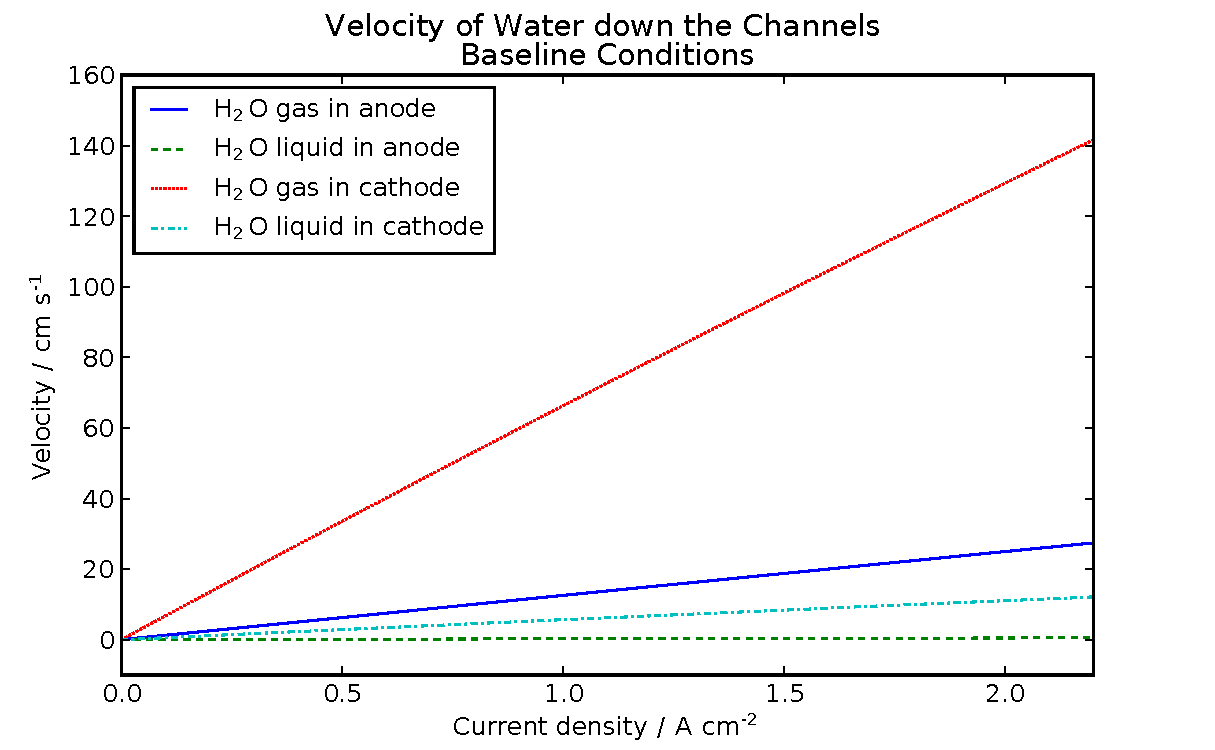
\includegraphics[width=\linewidth]{Results/Cell/Model/1/Velocity}%
  \caption{Velocity of \s{H2O} down the channels during the baseline polarization}%
  \label{fig:BaselineVelocity}
\end{figure}

The model also includes the pressures of individual gas species.  Figures~\ref{fig:PressureH2}, \ref{fig:PressureH2O}, and \ref{fig:PressureO2} show the pressures of \n{H2}, \n{O2}, and \n{H2O} along their primary transport paths.  The pressure of \n{H2} decreases from the anode inlet to the \n{HOR} and the pressure of \n{O2} decreases from the cathode inlet to the \n{ORR}.  The pressure of \n{H2O} drops from the \n{ORR} to the cathode outlet.

\begin{figure}[htbp]
  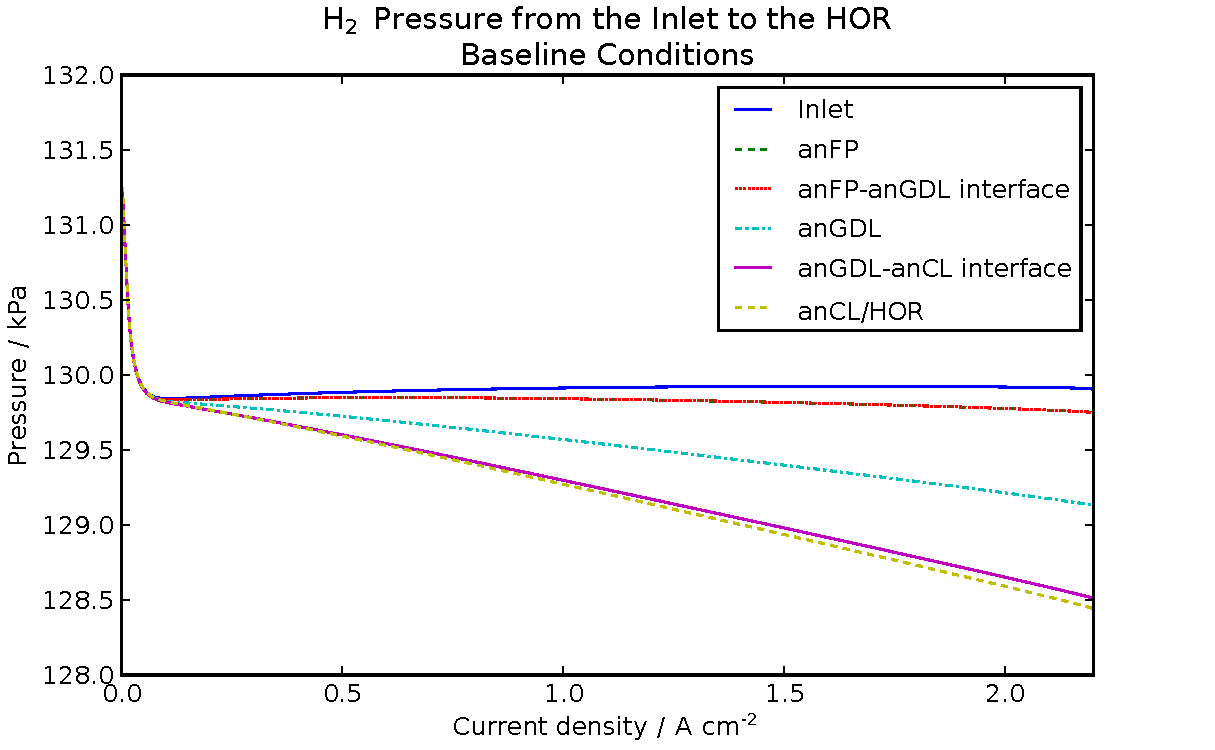
\includegraphics[width=\linewidth]{Results/Cell/Model/1/PressureH2}%
  \caption{\s{H2} pressure during the baseline polarization}%
  \label{fig:PressureH2}
\end{figure}

\begin{figure}[htbp]
  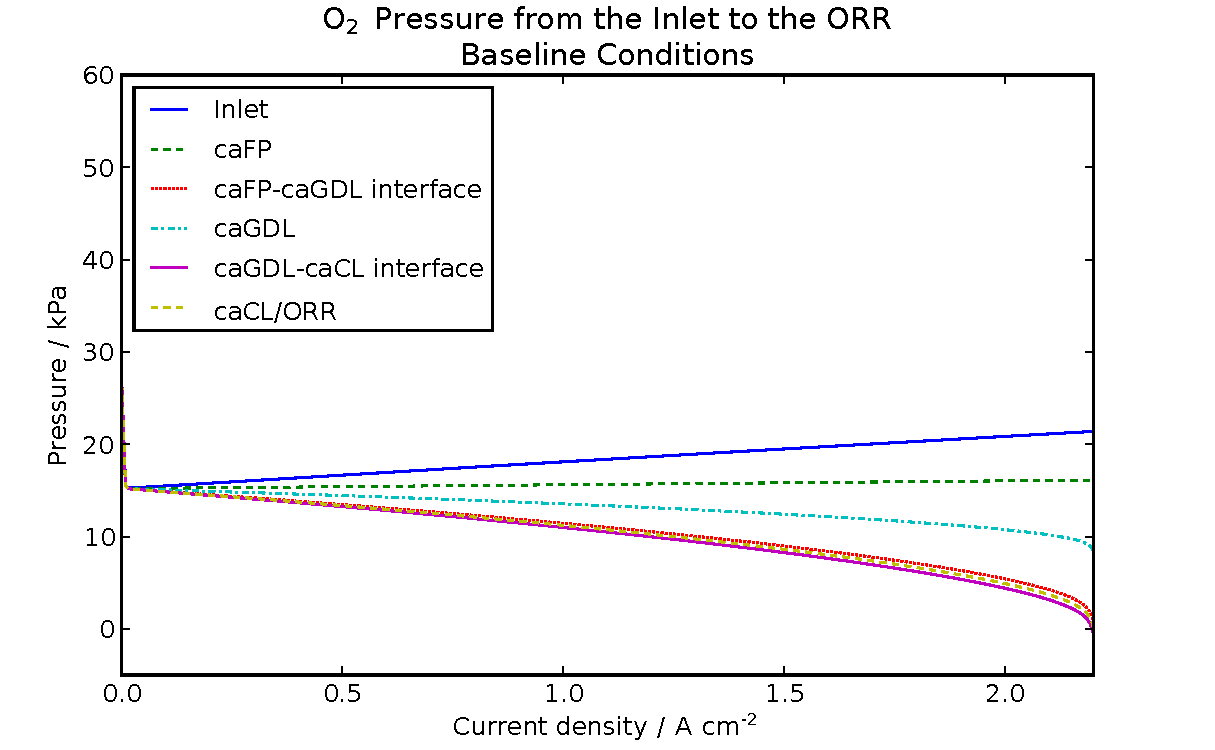
\includegraphics[width=\linewidth]{Results/Cell/Model/1/PressureO2}%
  \caption{\s{O2} pressure during the baseline polarization}%
  \label{fig:PressureO2}
\end{figure}

\begin{figure}[htbp]
  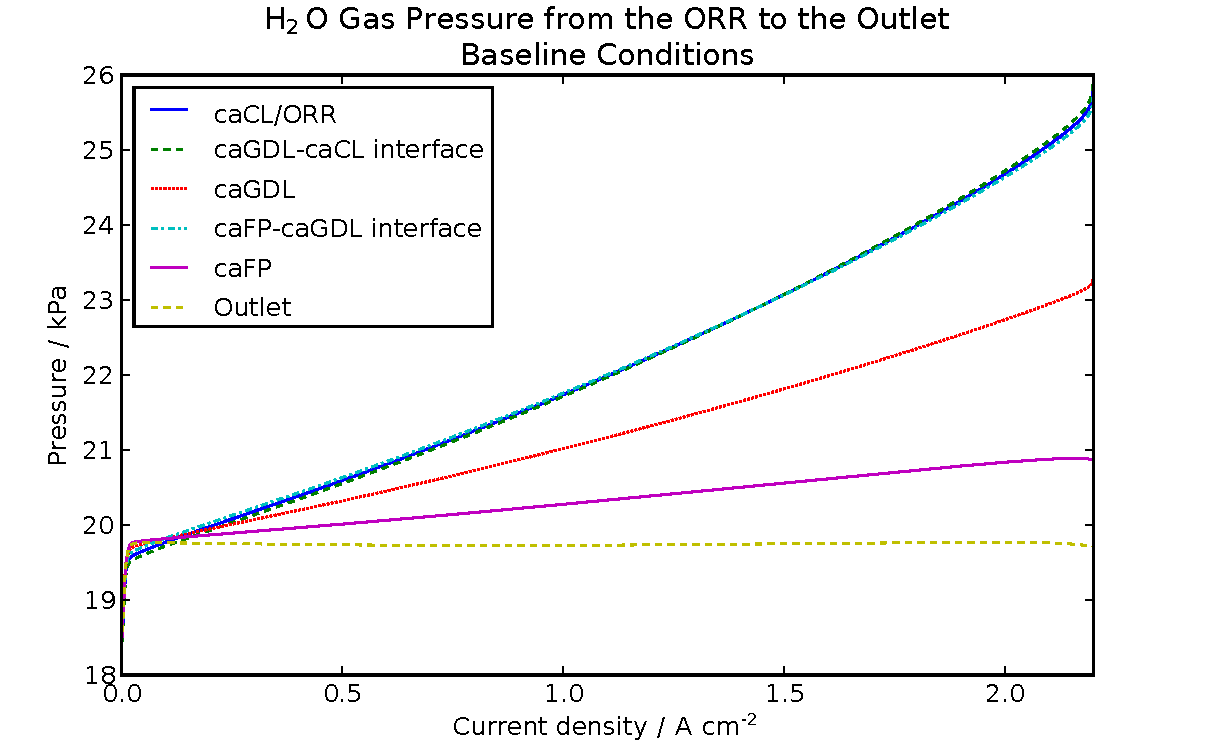
\includegraphics[width=\linewidth]{Results/Cell/Model/1/PressureH2O}%
  \caption{\s{H2O} pressure during the baseline polarization}%
  \label{fig:PressureH2O}
\end{figure}

Not all of the \n{H2O} exits from the cathode.  The Sankey diagram in \autoref{fig:BaselineWater} shows the water balance at \SI{1.5}{A/cm^2}.  Water is generated at the rate of \SI{37.5}{A/cm^2} ($\SI{1.5}{A/cm^2} \s{e-} \times \SI{50}{cm^2} \times 1 \s{H2O} / 2 \s{e-}$).  There is a net input of water vapor into the anode and a net output of liquid.  Water exits the cathode channels as gas and liquid.

\begin{figure}[htbp]
  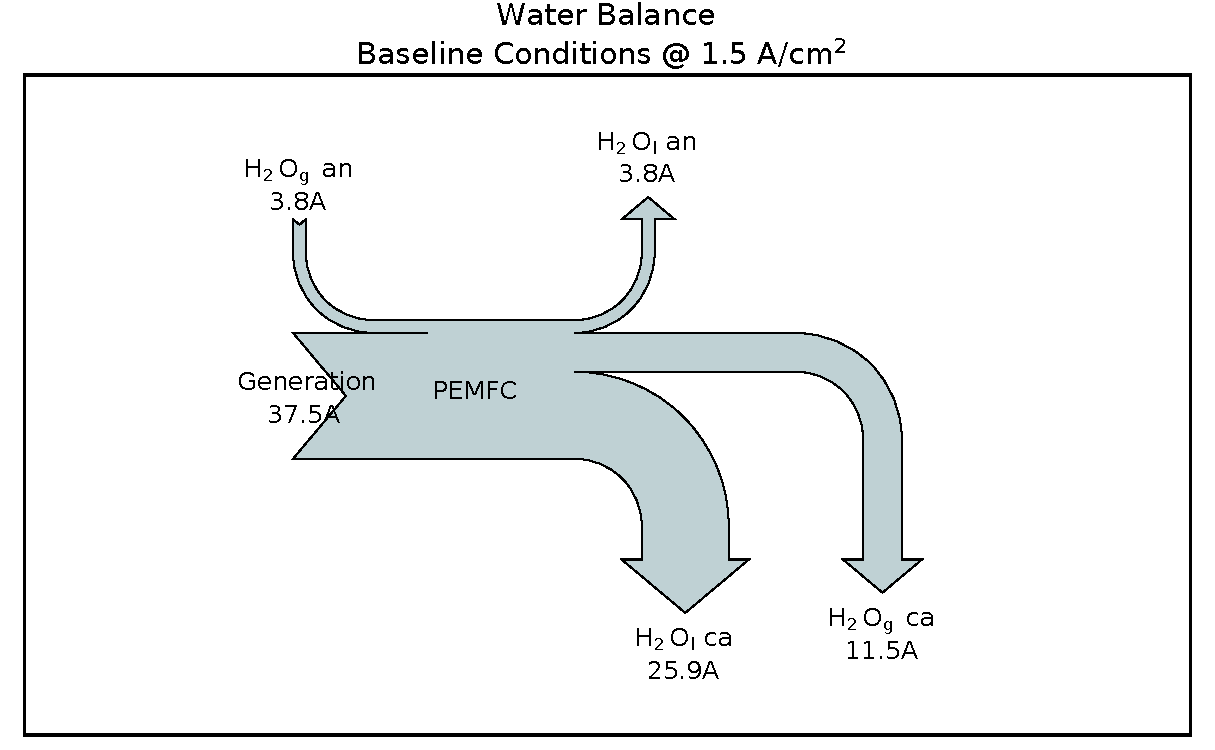
\includegraphics[width=\linewidth]{Results/Cell/Model/1/Water}%
  \caption{\s{H2O} balance under the baseline conditions at \SI{1.5}{A/cm^2}}%
  \label{fig:BaselineWater}
\end{figure}

\autoref{fig:H2OTransport} shows the transport of water through the layers.  It condenses near the interface of the anode flow plate and the anode \n{GDL} because it is super-saturated in the \n{GDL} relative to the channel due to the \n{GDL}'s hydrophobicity.  The current of water through the ionomer is relatively small, but as shown in \autoref{fig:H2OTransportPEM}, it is not zero.  At low currents ($<\SI{1}{A/cm^2}$), there is a fairly linear increase in the rate of transport through the \n{PEM} from the anode to the cathode due to the concentration gradient generated by the production of water in the cathode.  However, the electro-osmotic drag becomes significant at high electrical currents and counters the diffusion.  At the limiting current density, there is a rapid reversal of the trend caused by electro-osmotic drag because the cathode fills with liquid.

\begin{figure}[htbp]
  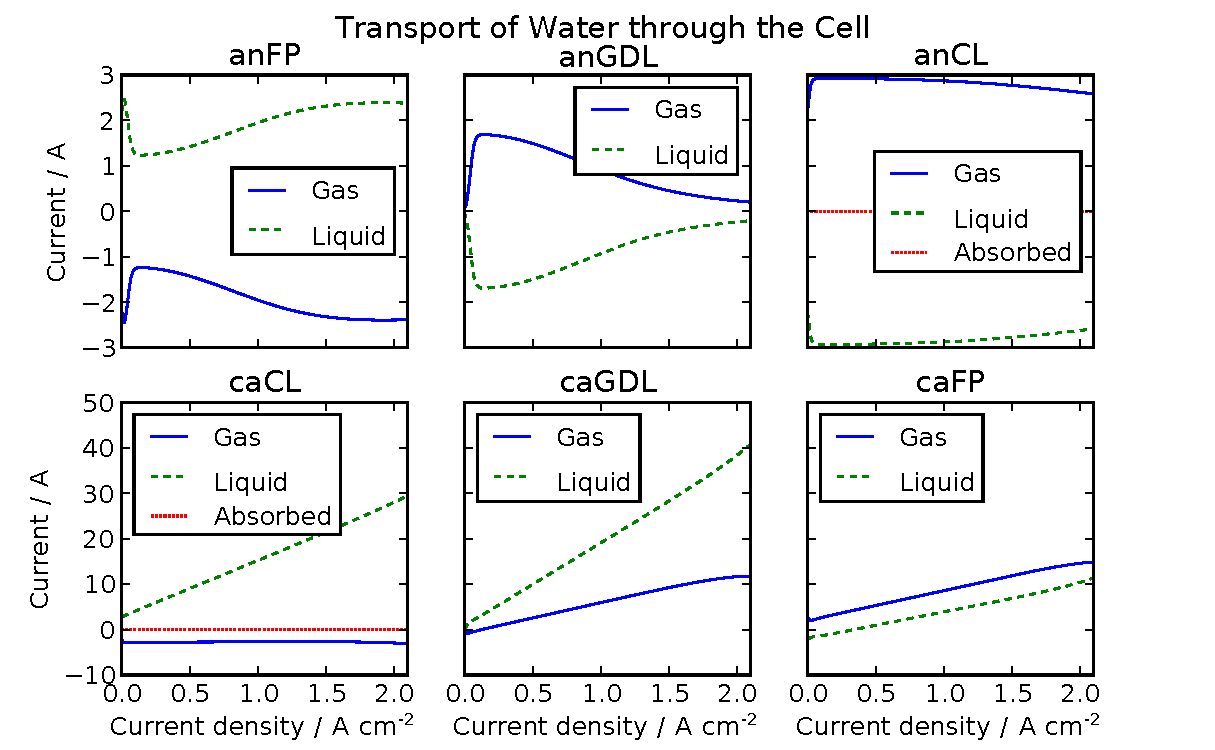
\includegraphics[width=\linewidth]{Results/Cell/Model/1/H2OTransport}%
  \caption{\s{H2O} transport during the baseline polarization}%
  \label{fig:H2OTransport}
\end{figure}

\begin{figure}[htbp]
  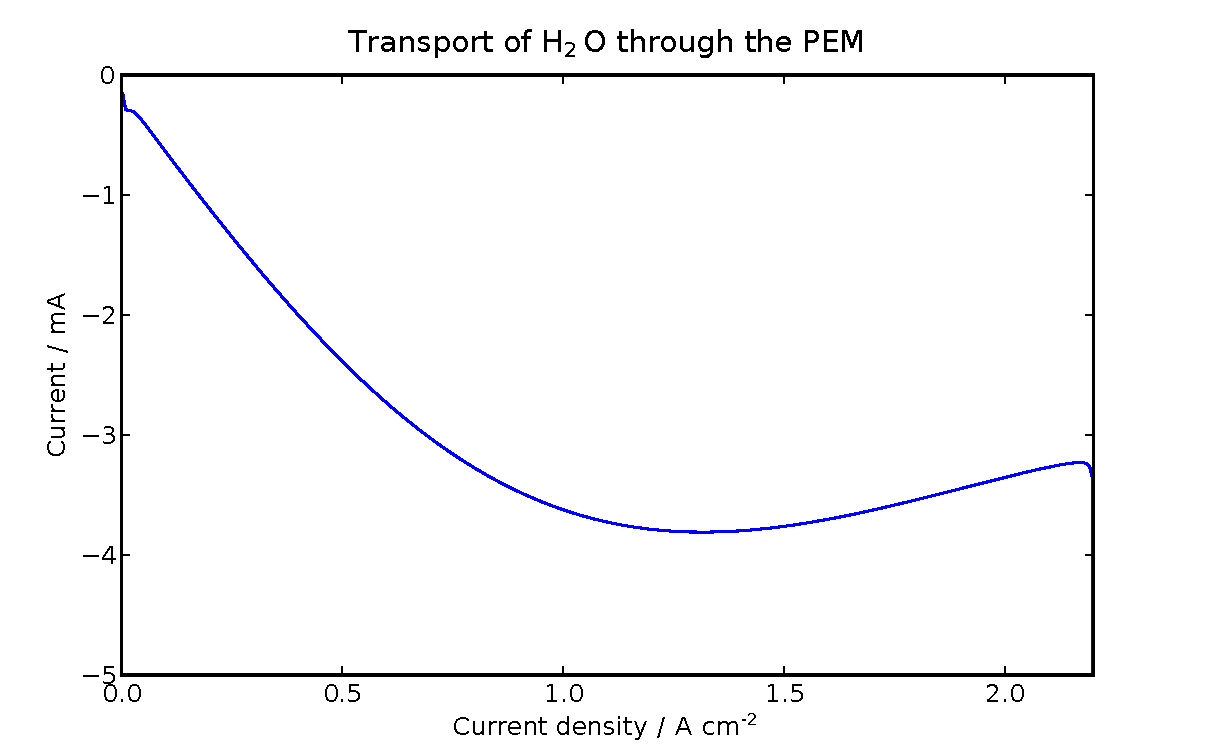
\includegraphics[width=\linewidth]{Results/Cell/Model/1/H2OTransportPEM}%
  \caption[\s{H2O} transport through the membrane during the baseline polarization]{\s{H2O} transport through the \n{PEM} during the baseline polarization}%
  \label{fig:H2OTransportPEM}
\end{figure}

\autoref{fig:BaselineHydration} shows the level of hydration in the ionomer of the catalyst layers and the \n{PEM}.  As the electrical current increases, water is produced more rapidly.  This increases the hydration, beginning in the cathode catalyst layer.  Although the concentration gradient is larger at higher electrical currents, so is the drag due to protonic transport.  As was seen in \autoref{fig:H2OTransportPEM}, the diffusion reaches a maximum (in magnitude) around \SI{1.3}{A/cm^2}.

\begin{figure}[htbp]
  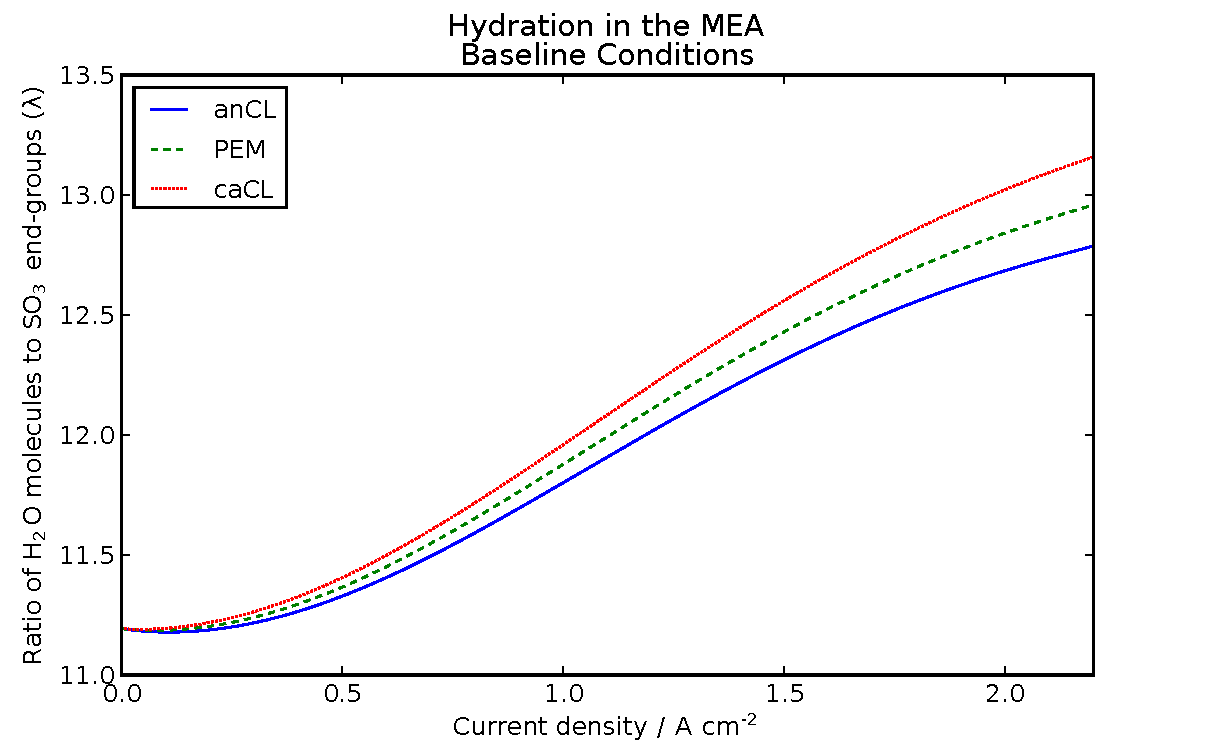
\includegraphics[width=\linewidth]{Results/Cell/Model/1/Hydration}%
  \caption[Hydration during the baseline polarization test]{Hydration of the \n{MEA} during the baseline polarization}%
  \label{fig:BaselineHydration}
\end{figure}

Besides entering the membrane, water also fills the pores of the cathode catalyst layer and \n{GDL}.  This is shown in \autoref{fig:PoreSaturation}.  At the limiting current density, the \n{GDL} pores are 45\% filled and rapidly filling further.  The catalyst layer retains water to a lesser extent.  The model assumes that the pores are smaller in the catalyst layer than the \n{GDL} (see \autoref{tab:CellParams}) but have the same hydrophobicity.  This yields a stronger capillary pressure, which tends to prevent flooding in the catalyst layer.

\begin{figure}[htbp]
  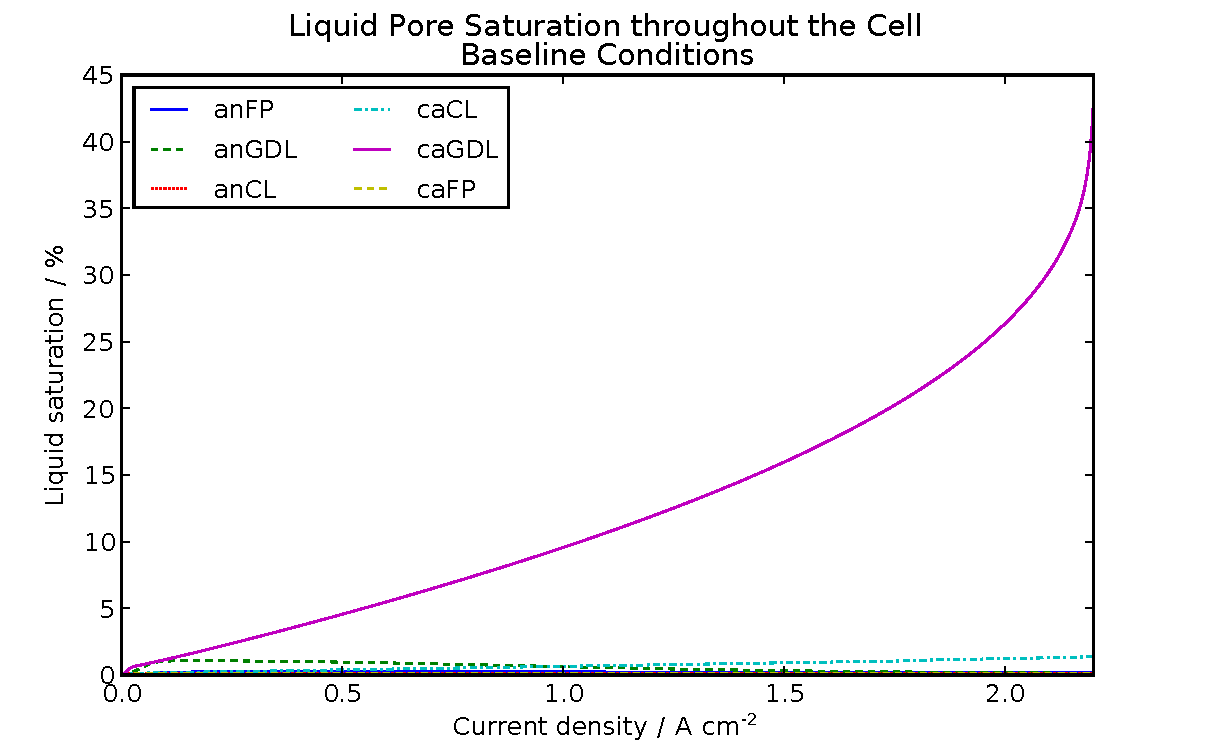
\includegraphics[width=\linewidth]{Results/Cell/Model/1/PoreSaturation}%
  \caption{Liquid pore saturation during the baseline polarization}%
  \label{fig:PoreSaturation}
\end{figure}

\autoref{fig:BaselineRH} shows the humidity throughout the cell.  The relative humidity is slightly higher than 100\% in the cathode channel because the water enters the channel from the catalyst layer and the \n{GDL}, which are hotter due to heat generation.  Also, the \n{GDL}  is modeled as hydrophobic, which implies a lower saturation pressure (i.e., the Kelvin equation) such that saturated vapor in the \n{GDL} is supersaturated in the channel (even at the same temperature).  The vapor in the anode flow plate is saturated, but it appears slightly below 100\% relative humidity.  The reason is that the relative humidity is only an output\slash{}analysis variable in the model.  It is calculated from \modelica{Modelica.Media.Air.MoistAir.saturationPressure()}, which does not correspond exactly to the model.  This was apparent in \autoref{fig:SaturationPressure}.

\begin{figure}[htbp]
  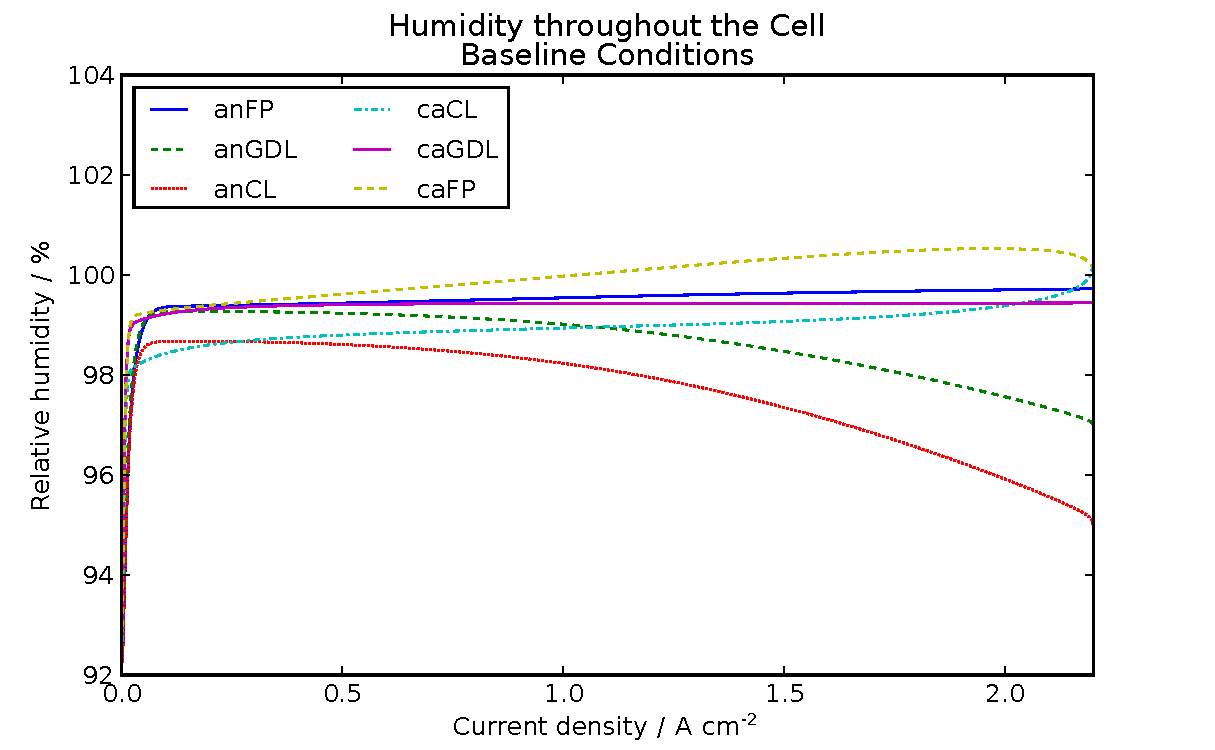
\includegraphics[width=\linewidth]{Results/Cell/Model/1/Humidity}%
  \caption{Relative humidity through the cell during the baseline polarization}%
  \label{fig:BaselineRH}
\end{figure}

\autoref{fig:EvaporationRateCell} shows the rates of evaporation throughout the cell.  Water evaporates most rapidly in the cathode catalyst layer.  The \n{ORR} is modeled as producing liquid, not vapor, and the liquid evaporates to reach saturation.  Water condenses in the other layers.  The largest rate is in the cathode channel.

\begin{figure}[htbp]
  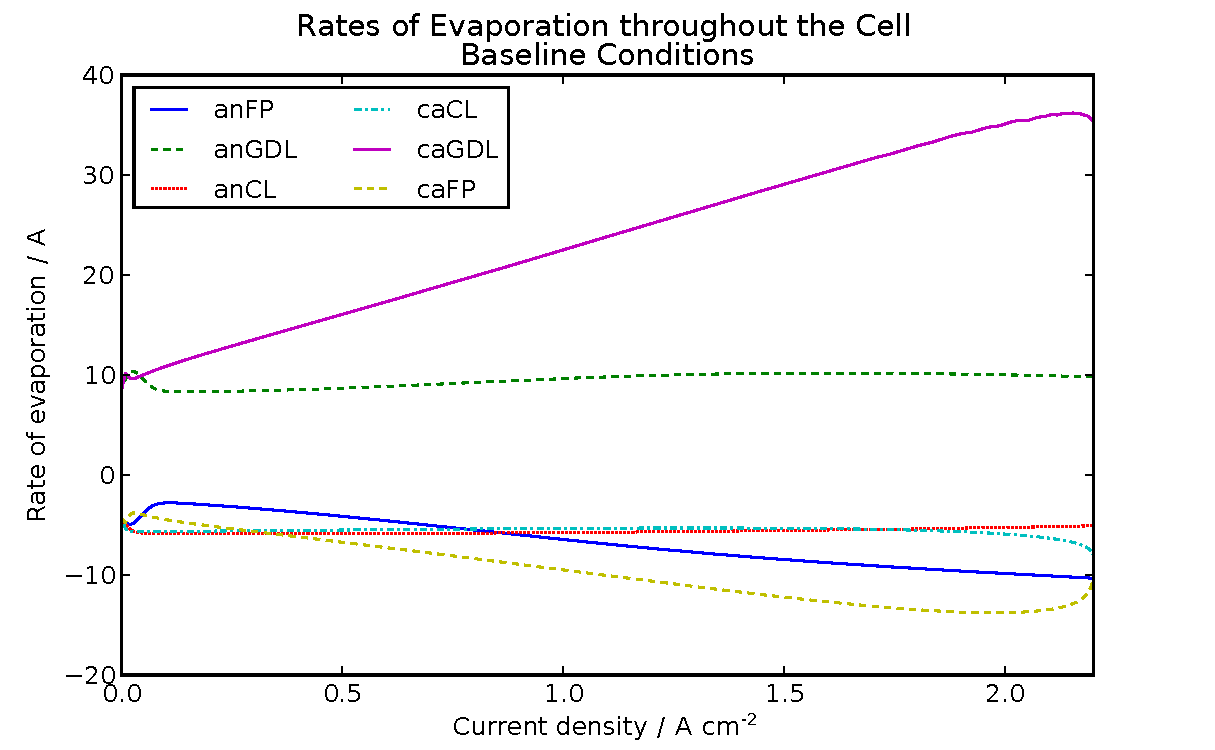
\includegraphics[width=\linewidth]{Results/Cell/Model/1/EvaporationRate}%
  \caption{Rates of evaporation during the baseline polarization}%
  \label{fig:EvaporationRateCell}
\end{figure}

\autoref{fig:CellHydrationRate} shows the rates of hydration in the catalyst layers.  Water is absorbed on the cathode side and desorbed on the anode side where the relative humidity is lower (see \autoref{fig:BaselineRH}) and there is evaporation (see \autoref{fig:EvaporationRateCell}).  Note, however, that the rate of hydration is much slower than the rate of evaporation.  This is consistent with the examples in the last two sections of \autoref{chap:Basic}.

\begin{figure}[htbp]
  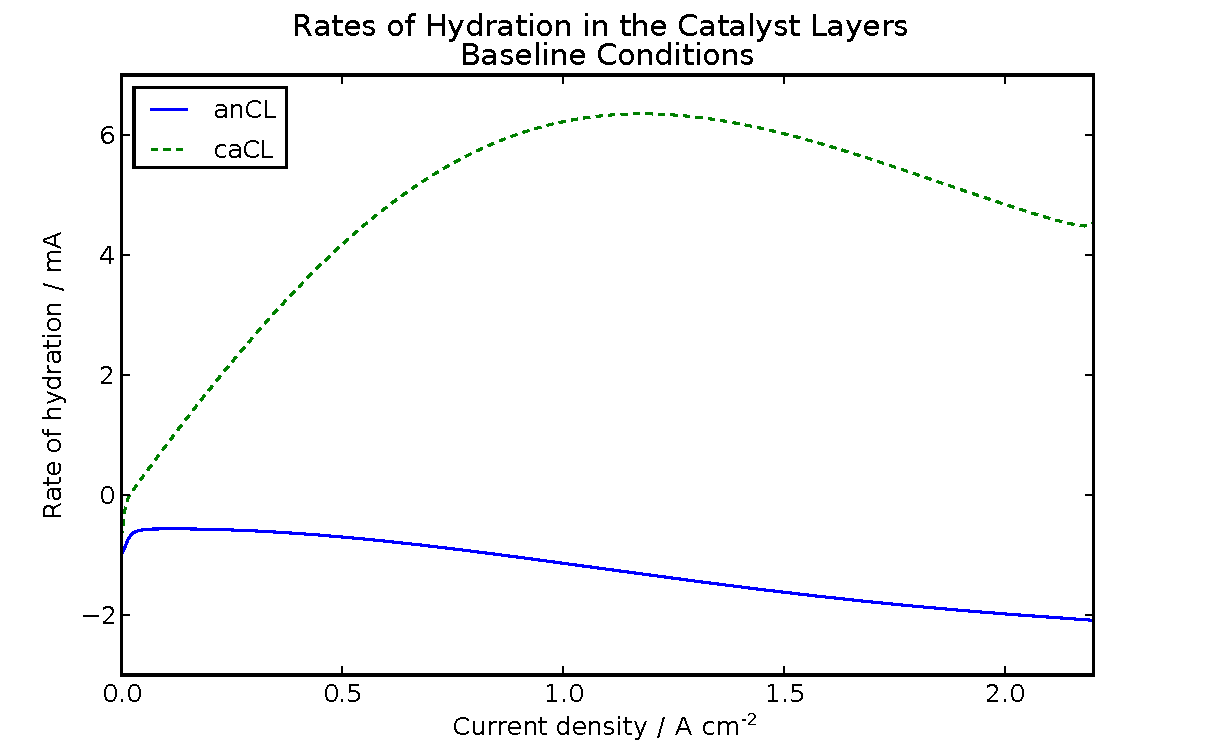
\includegraphics[width=\linewidth]{Results/Cell/Model/1/HydrationRate}%
  \caption{Rates of hydration during the baseline polarization}%
  \label{fig:CellHydrationRate}
\end{figure}


\FloatBarrier % Flush the floats.
\section{Varying Temperature}
\label{sec:Temperature}

\subsection{Conditions}

The temperature of the polarization test is changed to 40 and \SI{80}{\celsius} from the 
baseline of \SI{60}{\celsius}.  As mentioned in \autoref{sec:Baseline-Conditions}, the selected temperature is applied to the reactant supples, the exterior x-axis boundaries of the flow plates, and the initial conditions of the cell.  All other settings are the same as for the baseline test (previous section).

\subsection{Results and Discussion}

The model statistics (numbers of both types of variables, number of states, and number of systems of equations) are the same as for the baseline test and the computation times are nearly the same.  Unfortunately, the modeling tool requires that the model be re-translated when the temperature condition is changed.  Sometimes this is necessary when a parameter has implications that may affect the structure of the underlying equations.

\autoref{fig:TemperaturePolarization} compares the polarization of the model against the experimental data.  The same issues are apparent as in \autoref{sec:Baseline-Results}: the model over-predicts the activation region, under-predicts the Ohmic region, and does not show a gradual enough roll-off in the concentration region.  The model does capture the trend towards higher performance at higher temperatures, but not to the extent of the experimental cell.

\begin{figure}[htbp]
  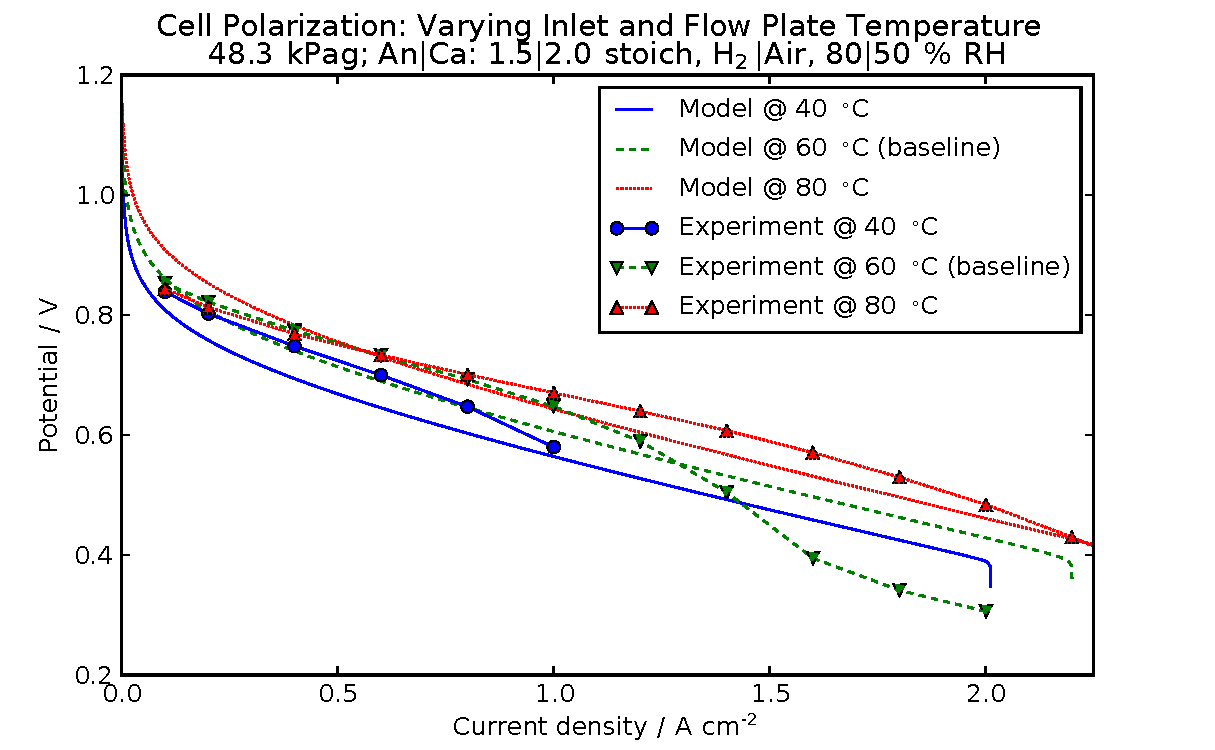
\includegraphics[width=\linewidth]{Results/Cell/Model/Temperature/Polarization}%
  \caption{Polarization curves with varying temperature}%
  \label{fig:TemperaturePolarization}
\end{figure}



\FloatBarrier % Flush the floats.
\section{Varying Pressure}

\subsection{Conditions}

The pressure of the polarization test is changed to 0 and \SI{202.7}{kPag} from the 
baseline of \SI{48.3}{kPag}.  The selected pressure is applied to both of the outlets and to the initial conditions.  All other settings are the same as for the baseline test (\autoref{sec:Baseline}).

\subsection{Results and Discussion}

The model statistics are the same as for the baseline test and the computation times are nearly the same.  Unfortunately, the modeling tool requires that the model be re-translated when the pressure is changed.

\autoref{fig:PressurePolarization} compares the polarization of the model against the experimental data.  The same general issues exist as before.  The model does capture the trend towards higher performance at higher pressure, but not to the extent of the experimental cell.

\begin{figure}[htbp]
  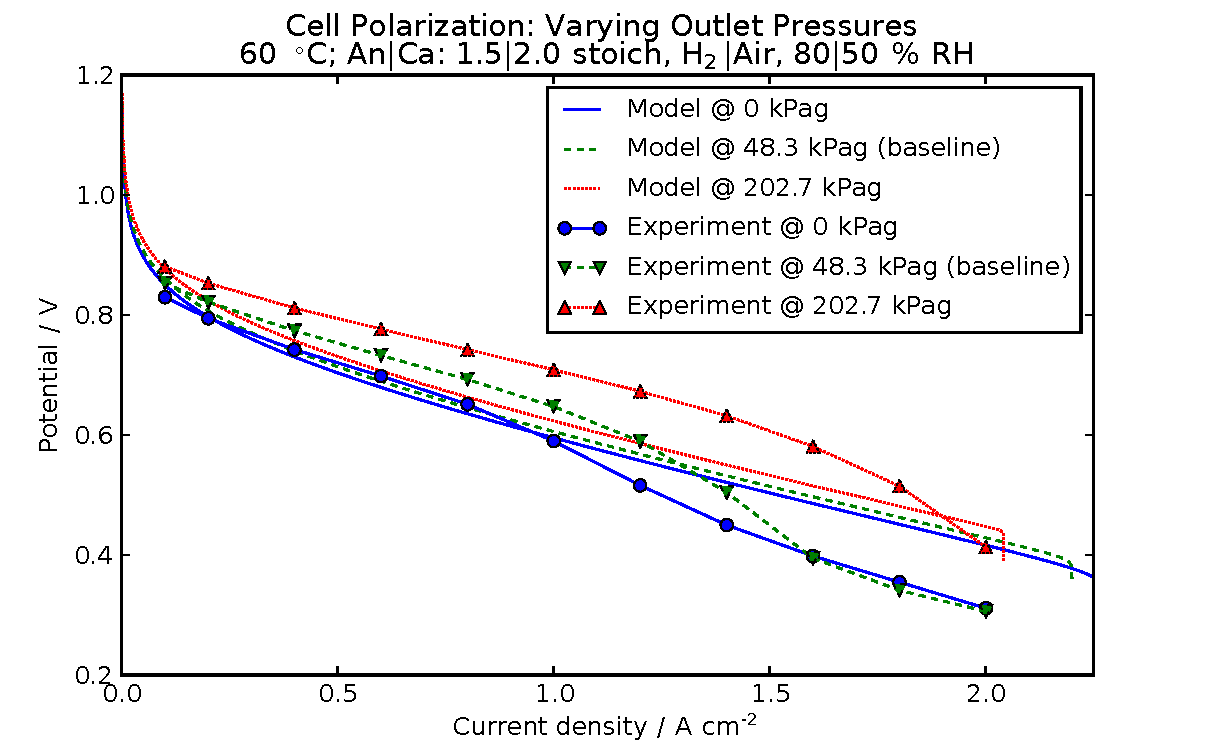
\includegraphics[width=\linewidth]{Results/Cell/Model/Pressure/Polarization}%
  \caption{Polarization curves with varying outlet pressure}%
  \label{fig:PressurePolarization}
\end{figure}


\FloatBarrier % Flush the floats.
\section{Varying Anode Flow Rate}

\subsection{Conditions}

The anode stoichiometric flow rate of the polarization test is changed to 1.1 and 2.0 from the 
baseline of 1.5.  All other settings are the same as for the baseline test (\autoref{sec:Baseline}).

\subsection{Results and Discussion}

The model statistics and translation time are the same as for the baseline test.  The simulation time is only slightly different.  It is possible to change the anode flow rate without re-translating the model.

\autoref{fig:AnFlowPolarization} compares the polarization of the model against the experimental data.  Although the same general issues exist as noted in \autoref{sec:Temperature}, the model and the experimental data both indicate that anode flow rate has little effect on the polarization.  The supply of hydrogen generally does not limit the operation of the cell.  The cathode supply does.

\begin{figure}[htbp]
  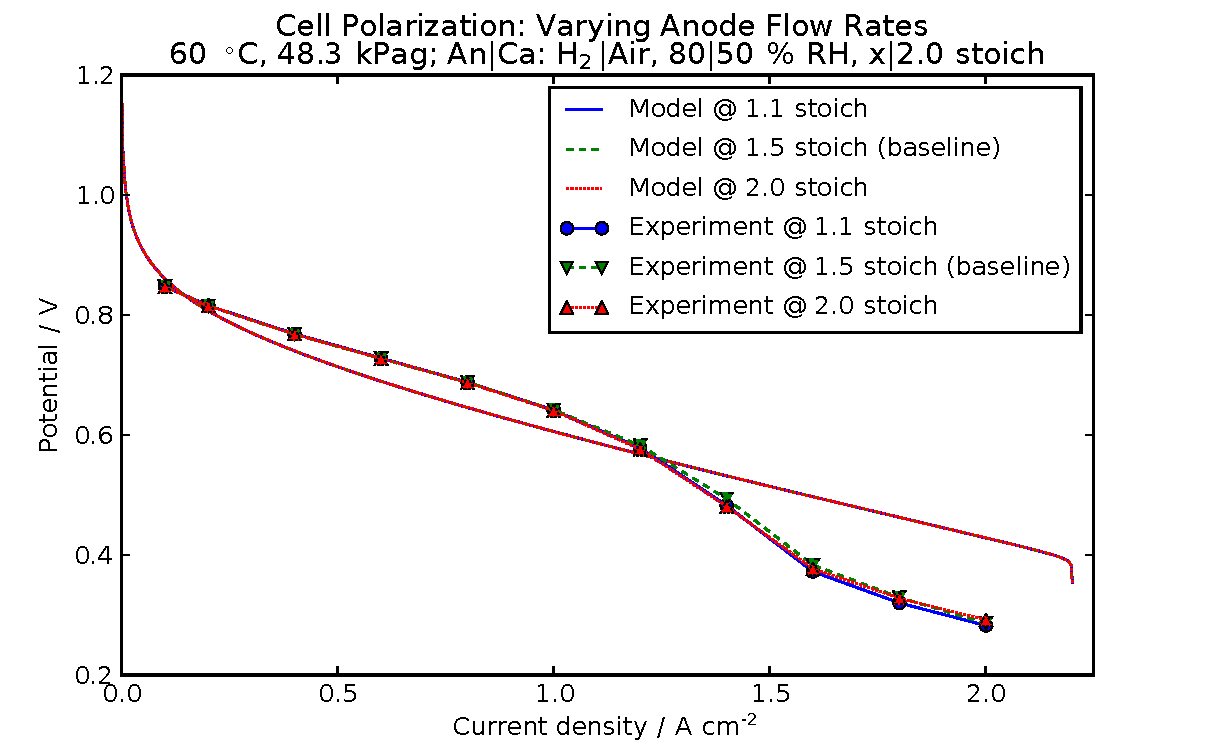
\includegraphics[width=\linewidth]{Results/Cell/Model/AnFlow/Polarization}%
  \caption{Polarization curves with varying anode flow rates}%
  \label{fig:AnFlowPolarization}
\end{figure}


\FloatBarrier % Flush the floats.
\section{Varying Cathode Flow Conditions}

\subsection{Conditions}

The cathode stoichiometric flow rate of the polarization test is changed to 1.5 and 2.5 from the 
baseline of 2.0.  In addition, the supply is changed to \s{O2} (no \n{N2}) and the cell is operated at cathode stoichiometric flow rates of 7.177, 9.569, and 11.962.  All other settings are the same as for the baseline test (\autoref{sec:Baseline}).

\subsection{Results and Discussion}

The model statistics and translation time are the same as for the baseline test.  The simulation time is nearly the same.  It is possible to change the cathode flow rate without re-translating the model.  However, the choice of air or \n{O2} requires re-translation.

\autoref{fig:CaFlowPolarization} compares the polarization of the model against the experimental data.  In the case of air (\autoref{fig:CaFlowPolarizationAir}), the effect shown by the model is much less than the effect in the experimental data.  The model is affected very little in the Ohmic region, but the limiting current density changes considerably.  In the case of \s{O2} (\autoref{fig:CaFlowPolarizationO2}), the resistance should decrease significantly in the Ohmic region, but the model does not show it.  As was shown in Figures~\ref{fig:BaselineVoltages} and \ref{fig:BaselineElectricalLosses}, the resistance is dominated by protonic transport through the \n{PEM}.  The protonic resistance does not appear to change in the model.  The only way for it to change is for \begin{inparaenum}[(1)]\item the mobility factors to change (they are currently fixed) or \item the hydration of the \n{PEM} to change, affecting the degree of electro-osmotic drag.\end{inparaenum}

\begin{figure}[htbp]
  \subfloat[Air]{
    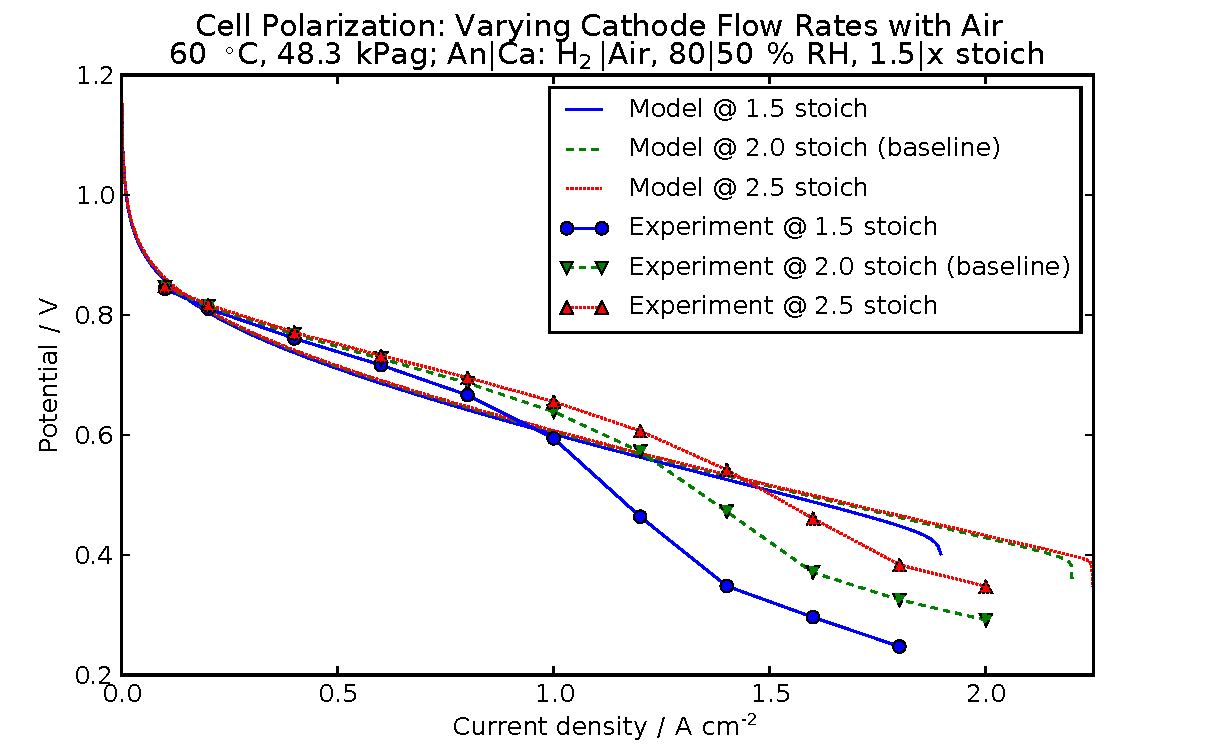
\includegraphics[width=\linewidth]{Results/Cell/Model/CaFlowAir/Polarization}%
    \label{fig:CaFlowPolarizationAir}
  }\quad
  \subfloat[Oxygen]{
    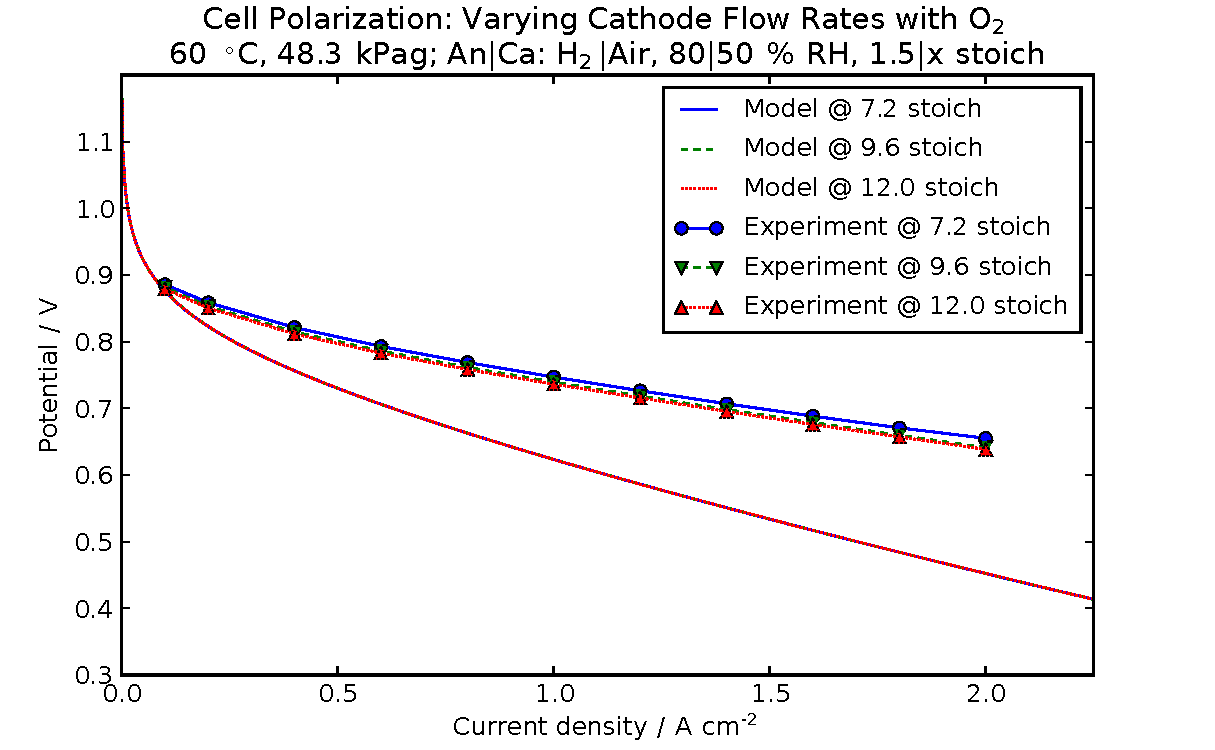
\includegraphics[width=\linewidth]{Results/Cell/Model/CaFlowO2/Polarization}%
    \label{fig:CaFlowPolarizationO2}
  }
  \caption{Polarization curves with varying cathode flow rates and compositions}%
  \label{fig:CaFlowPolarization}
\end{figure}


\FloatBarrier % Flush the floats.
\section{Varying Anode Humidity}

\subsection{Conditions}

The relative humidity of the anode supply is changed to 60 and 100\% from the 
baseline of 80\%.  All other settings are the same as for the baseline polarization test (\autoref{sec:Baseline}).

\subsection{Results and Discussion}

The model statistics are the same as for the baseline test and the computation times are nearly the same.  The modeling tool requires that the model be re-translated when the humidity of the anode supply is changed.  

The anode humidity has little effect on the polarization, as shown in \autoref{fig:AnHumidityPolarization} for both the model and the experimental cell.

\begin{figure}[htbp]
  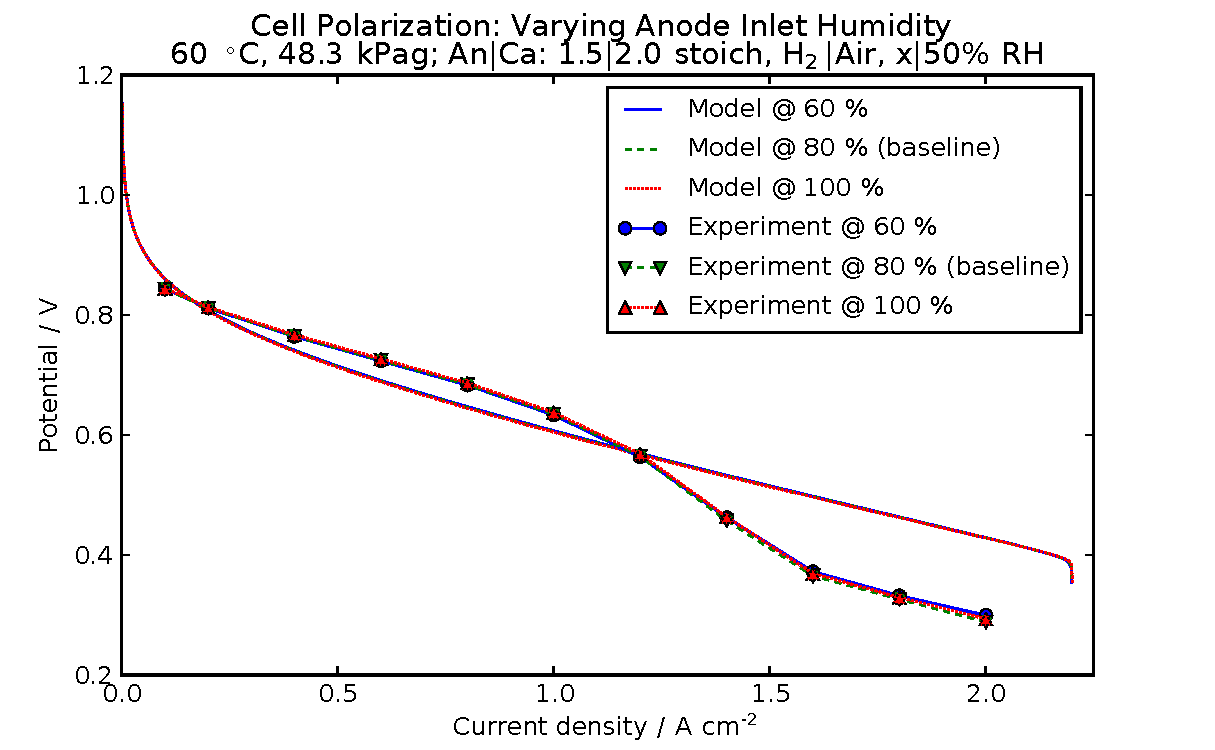
\includegraphics[width=\linewidth]{Results/Cell/Model/AnHumidity/Polarization}%
  \caption{Polarization curves with varying humidity at the anode inlet}%
  \label{fig:AnHumidityPolarization}
\end{figure}


\FloatBarrier % Flush the floats.
\section{Varying Cathode Humidity}
\label{sec:CaHumidity}

\subsection{Conditions}

The relative humidity of the cathode supply is changed to 30 and 70\% from the 
baseline of 50\%.  All other settings are the same as for the baseline polarization test (\autoref{sec:Baseline}).

\subsection{Results and Discussion}

The model statistics and translation time are the same as for the baseline test and the simulation time is nearly the same.  The humidity of the cathode supply can be changed without re-translating the model.  

As shown in \autoref{fig:CaHumidityPolarization}, the cathode humidity has a slight effect on the polarization of the experimental cell in the concentration region.  This reinforces the hypothesis that the rapid decrease in voltage from 1.0 to \SI{1.5}{A/cm^2} is due to the presence of liquid water.  It may be the case that the water begins to fill the pores of the cathode \n{GDL} and then is released (possibly by a capillary effect or by the flow of vapor from the catalyst layer) above \SI{1.5}{A/cm^2}.  As was shown in \autoref{fig:PoreSaturation}, liquid does fill the pores of the cathode \n{GDL} in the model.  This increases the pressure gradient required for a given rate of \n{O2} transport.  However, it seems that that only affects the limiting current density.  It does not introduce a recoverable concentration roll-off.

\begin{figure}[htbp]
  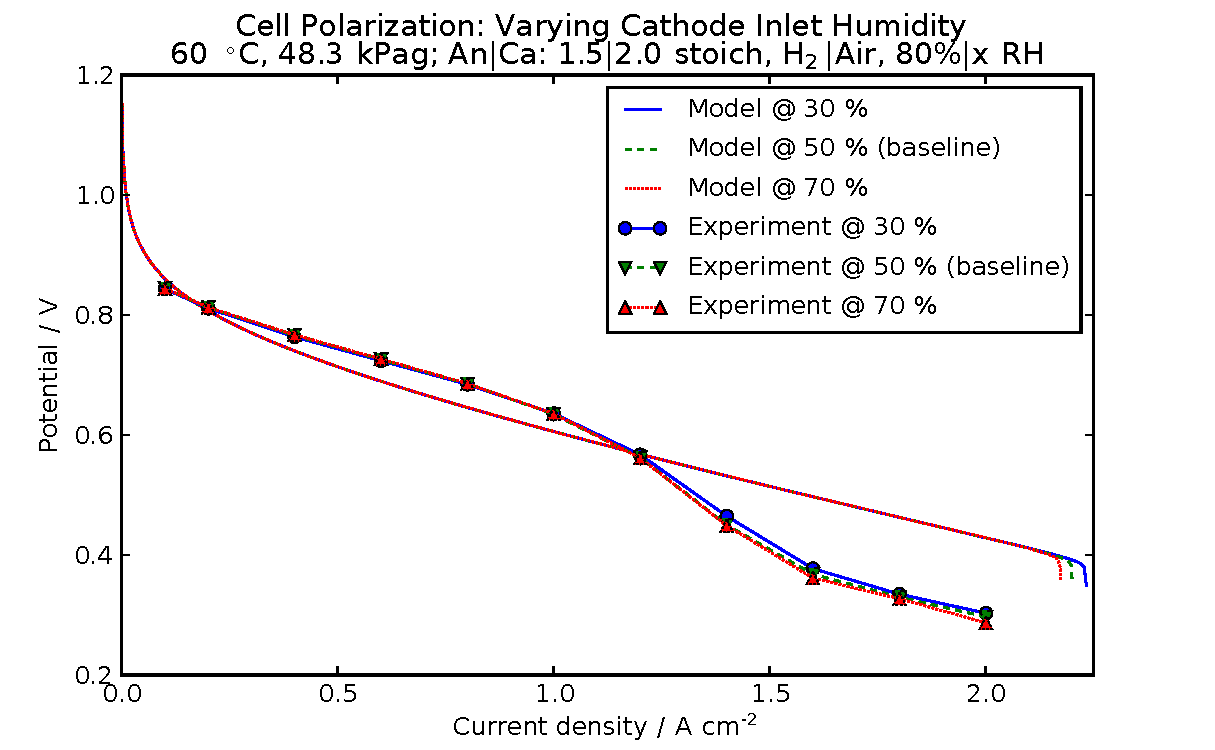
\includegraphics[width=\linewidth]{Results/Cell/Model/CaHumidity/Polarization}%
  \caption{Polarization curves with varying humidity at the cathode inlet}%
  \label{fig:CaHumidityPolarization}
\end{figure}


\FloatBarrier % Flush the floats.
\section{Simple Cell Model}
\label{sec:SimpleCell}

A simplified fuel cell model is tested under the baseline conditions in order to establish a lower limit on the complexity of the model and the computation time.  

\subsection{Conditions}

As discussed in \autoref{chap:Implementation}, the simple cell model assumes the same temperature for all phases in each flow plate.  This is in addition to the assumption in the standard cell model that all phases have the same temperature in the \np{GDL} and catalyst layers.  Liquid water is not included, and the \n{ORR} produces vapor instead of liquid.  The \n{GDL} and catalyst layers are combined as shown in \autoref{fig:SimpleCellModel}.  In order to make the losses roughly the same as for the standard model, it was necessary to decrease the porosity of the combined layers to 0.16 (from 0.8).  Also, the mobility factor between \s{H+} and \s{H2O} was increased to 1 (from 0.02) and the protonic conductivity was increased to \SI{0.8}{S/cm} (from \SI{0.1}{S/cm}) in the combined layers (\n{PEM} unchanged).

The same base \modelica{TestStand} model (\autoref{fig:TestStandD}) is used for this example, but its cell is replaced by the simple cell model.

\subsection{Results and Discussion}

\begin{table}[h]
  \caption{Modeling and simulation statistics for the simple fuel cell model}
  \label{tab:SimpleStatistics}
  \begin{singlespaced}%
    \begin{tabular}{llll}%
        \toprule 
      & Standard model & \multicolumn{2}{c}{Simple model} \\
      \cmidrule{3-4}
      & (with analysis) & w/ analysis & w/o analysis \\
        \midrule
      Number of variables & 6887 & 4462 & 3564 \\
      Number of time-varying variables & 2749 & 1650 & 866 \\
      Number of states & 55 & 27 & 27 \\
      Sizes of the nonlinear systems of equations & None & None & None \\
      Translation time & \SI{23}{s} & \SI{18}{s} & \SI{15}{s} \\
      Simulation time & \SI{1.56}{s} & \SI{0.222}{s} &  \SI{0.201}{s} \\
      \bottomrule
    \end{tabular}
  \end{singlespaced}
\end{table}


As listed in \autoref{tab:SimpleStatistics}, the simplified cell model has 35\% fewer total variables, 40\% fewer time-varying variables, and roughly half of the number of states.  It translates slightly more quickly than the standard model and simulates approximately seven times more quickly.  The complexity of the model can be decreased further by disabling the analysis variables.  Although this significantly decreases the number of time-varying variables, it does not affect the number of states.  Therefore, there is only a slight~(9\%) improvement in simulation time.  The model could be simplified yet further by setting the thermal resistivities to zero, yielding an isothermal, lumped-capacitance cell.

\autoref{fig:SimplePolarization} compares the polarization of the simple cell model against the standard cell model.  With the present parameter settings, the simple model has slightly less electrical resistance.  The concentration loss appears earlier and more gradually, which is actually desirable based on the experimental results (\autoref{sec:Baseline-Results}).

\begin{figure}[htbp]
  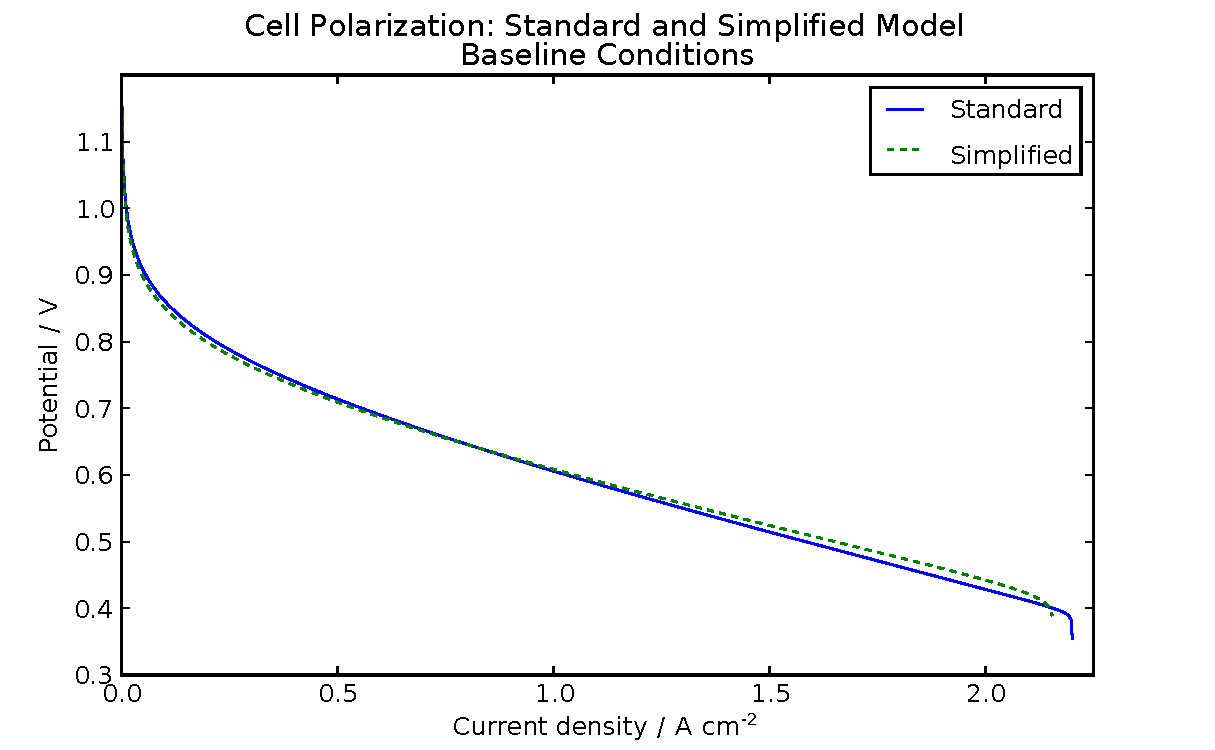
\includegraphics[width=\linewidth]{Results/Cell/Model/Simple/Polarization}%
  \caption{Polarization curves for the standard and simplified cell models}%
  \label{fig:SimplePolarization}
\end{figure}

Since liquid is not included, the relative humidity rises well above 100\%, as shown in \autoref{fig:SimpleHumidity}.  Another consequence of the exclusion of liquid is that the net hydration of the \n{MEA} is constant.  Since the hydration process is modeled as phase change between the liquid and the ionomer (not between gas and ionomer) and liquid is not included, water cannot enter or exit the ionomer.  

\begin{figure}[htbp]
  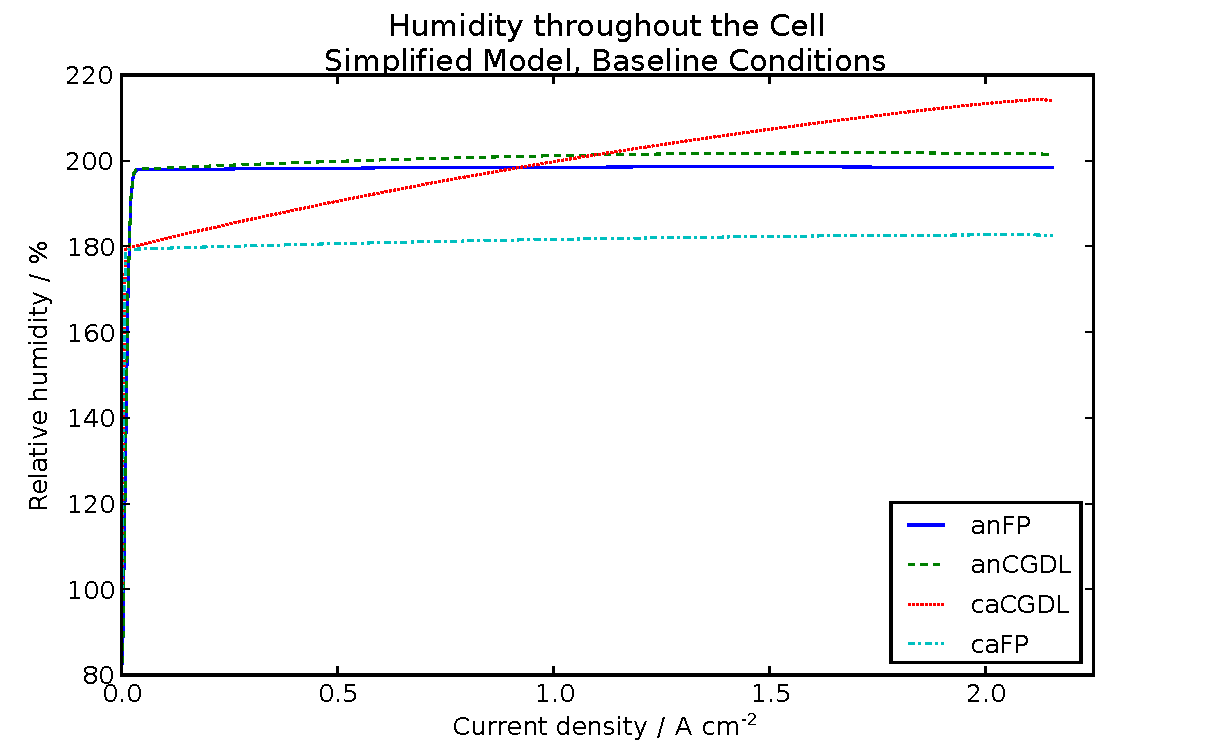
\includegraphics[width=\linewidth]{Results/Cell/Model/Simple/Humidity}%
  \caption{Relative humidity throughout the simplified cell model}%
  \label{fig:SimpleHumidity}
\end{figure}


\FloatBarrier % Flush the floats.
\section{Segmented Cell}
\label{sec:SegCell}

\subsection{Conditions}

In this section, a more complex configuration is considered by increasing the number of channel segments.  A version of the standard fuel cell model is created with six subregions down the length of the channel (y direction).  The electrical load is placed on the first segment, but the boundary temperature (\SI{60}{\celsius}) is applied to all of the segments.  Liquid water is disabled.  In order to make the losses without liquid roughly the same as for the standard model with liquid, it is necessary to change the porosity of the \np{GDL} to 0.45 (from 0.8).  The cell is operated under two conditions: the baseline conditions (\autoref{sec:Baseline-Conditions}) and the baseline conditions modified for fixed flow rates.  The fixed flows are given by \n{equivalent current} densities of 2.4 and \SI{3.2}{A/cm^2} in the anode and cathode, respectively.

\subsection{Results and Discussion}

\begin{table}[ht!]
  \caption{Modeling and simulation statistics for the segmented fuel cell model}
  \label{tab:SegmentedStatistics}
  \begin{singlespaced}%
    \begin{tabular}{llll}%
      \toprule 
      & \multicolumn{2}{c}{Stoichiometric flow} & \multicolumn{1}{c}{Fixed flow} \\
      \cmidrule{2-3}
      & w/ analysis & w/o analysis &  (w/ analysis) \\
      \midrule
      Number of variables & \num{31980} & \num{24835} & \num{31990} \\
      Number of time-varying variables & \num{12711} & \num{6547} & \num{12711} \\
      Number of states & 266 & 266 & 266 \\
      Sizes of the nonlinear systems of equations & None & None & None \\
      Translation time & \SI{67}{s} & \SI{48}{s} & \SI{69}{s} \\
      Simulation time & \SI{18.8}{s} & \SI{18.1}{s} & \SI{11.3}{s} \\
      \bottomrule
    \end{tabular}
  \end{singlespaced}
\end{table}


As listed in \autoref{tab:SegmentedStatistics}, the segmented cell model has approximately \num{32000} variables, roughly 40\% of which are time-varying.  There are approximately five times as many states as the standard, single-segment cell model.  There would be six times as many if liquid water were included.  As before, the analysis variables have little effect (4\%) on the simulation time.  The model runs 40\% more quickly under fixed flow conditions.

\autoref{fig:SegmentPolarizationNet} shows the net polarization of the model under the two flow regimes.  At \SI{1.6}{A/cm^2}, the supplies to the cell are equal under the stoichiometric and fixed flow conditions.  Until that point, the cell performs better under the fixed flow condition.  Shortly after that (at approximately \SI{1.8}{A/cm^2}), the cell begins to reach its concentration limit in the fixed flow example.

\begin{figure}[htbp]
  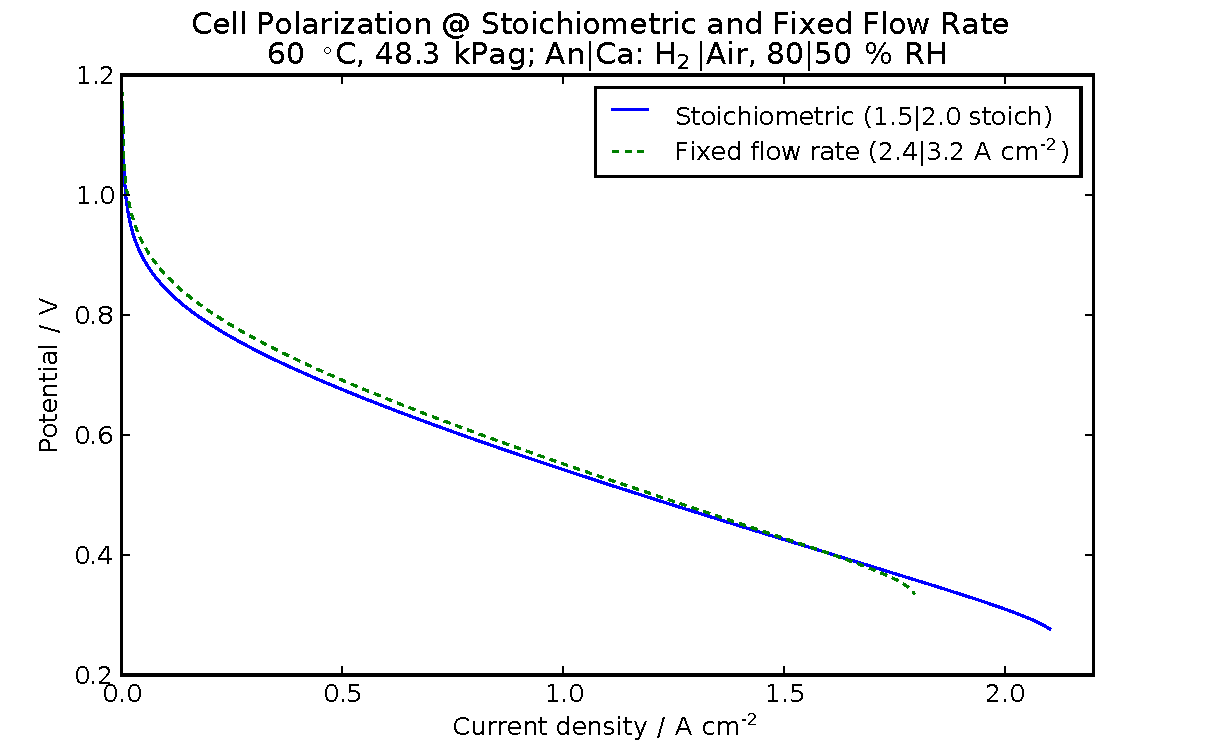
\includegraphics[width=\linewidth]{Results/Cell/Model/Segmented/Polarization}%
  \caption{Net polarization of the segmented cell under stoichiometric and fixed flow}%
  \label{fig:SegmentPolarizationNet}
\end{figure}

\autoref{fig:SegmentPolarization} shows the polarization of individual channel segments in the two operating regimes.  Cell potential is on the independent axis since it is nearly equal among the segments. The upstream segments perform better than the downstream ones because the \n{O2} pressure is higher there.  In the fixed flow example (\autoref{fig:SegmentPolarizationFixed}), the last segment begins to provide less current as more current is drawn from the entire cell above \SI{1.7}{A/cm^2}.  At that point, a positive feedback mechanism is established where an increase in net current requires more current from the upstream segments, further decreasing the \n{O2} available to the downstream segments.  The last segment is the first to become completely depleted of \n{O2}.  At that point, the simulation stops.

\begin{figure}[htbp]
  \subfloat[Anode]{
    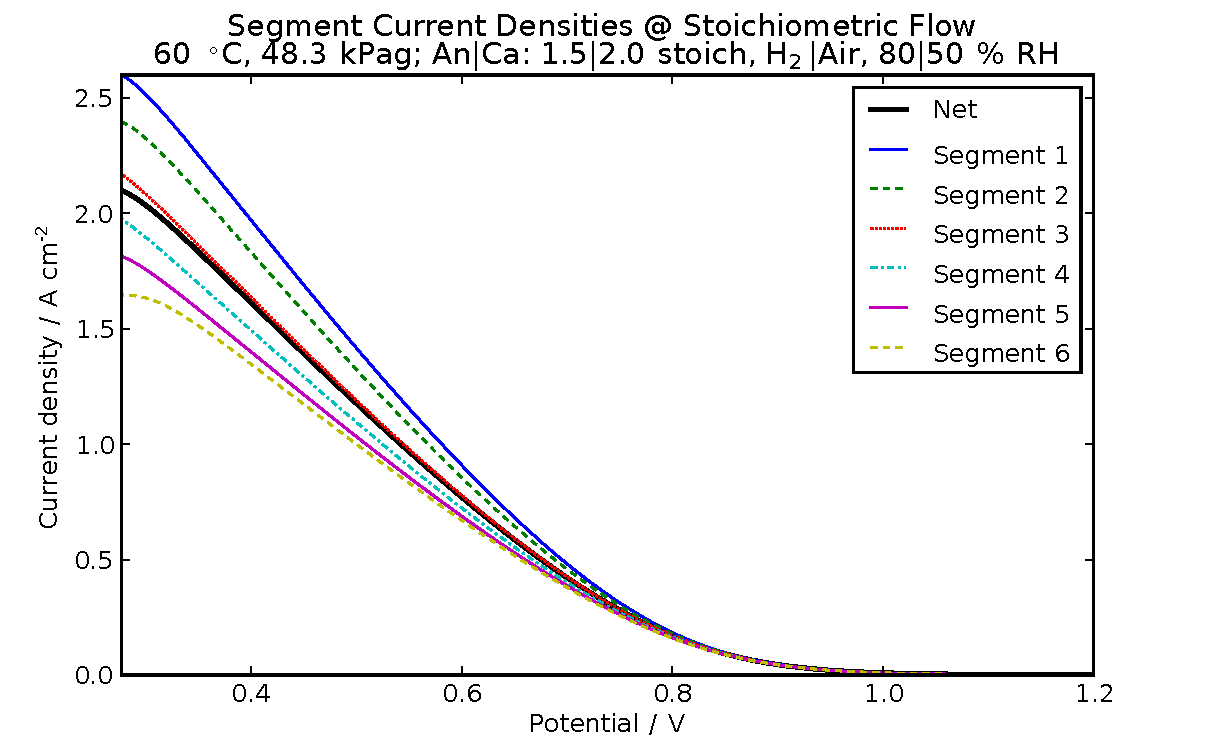
\includegraphics[width=\linewidth]{Results/Cell/Model/Segmented/PolarizationStoich}%
    \label{fig:SegmentPolarizationStoich}
  }\quad
  \subfloat[Cathode]{
    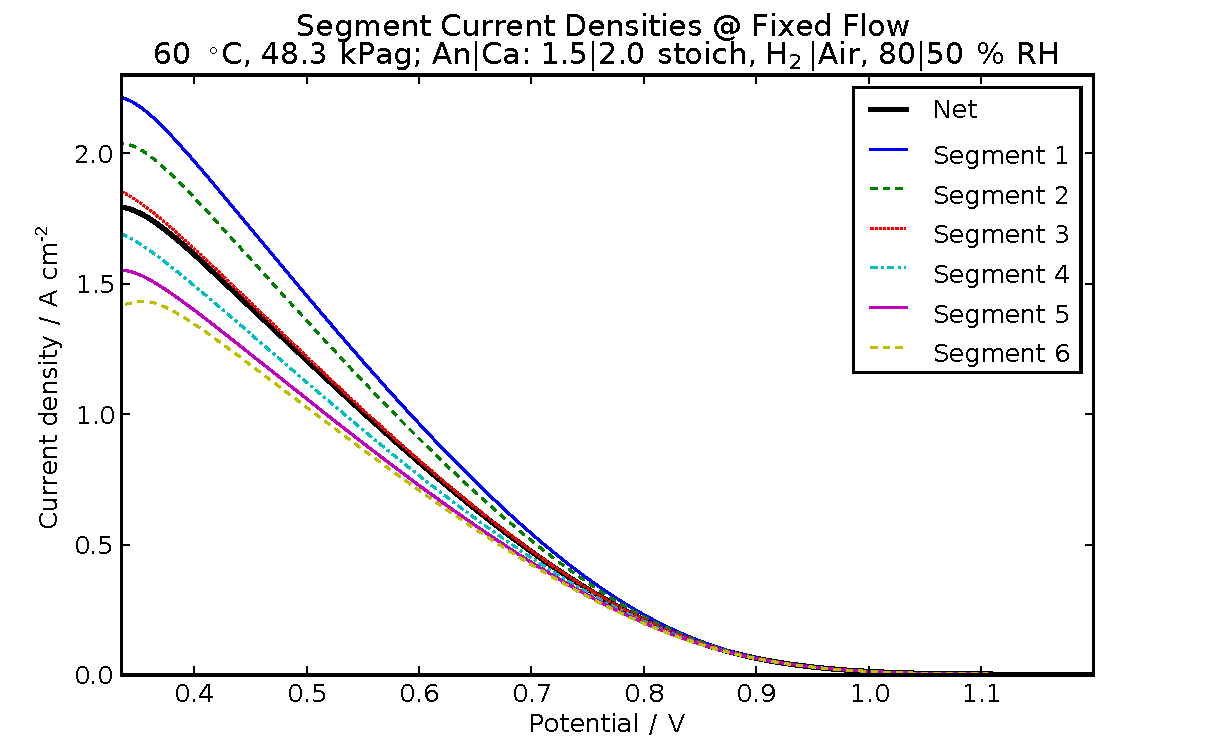
\includegraphics[width=\linewidth]{Results/Cell/Model/Segmented/PolarizationFixed}%
    \label{fig:SegmentPolarizationFixed}
  }
  \caption{Pressure down the channels of the segmented cell}%
  \label{fig:SegmentPolarization}
\end{figure}

\autoref{fig:SegmentO2Pressure} shows the \n{O2} pressure in the cathode catalyst layer under the stoichiometric flow conditions.  The pressure decreases fairly linearly with current density.  The downstream segments have lower pressures.  The pressure difference between the segments generally increases with current density because \n{O2} is consumed at a higher rate.

\begin{figure}[htbp]
  \fbox{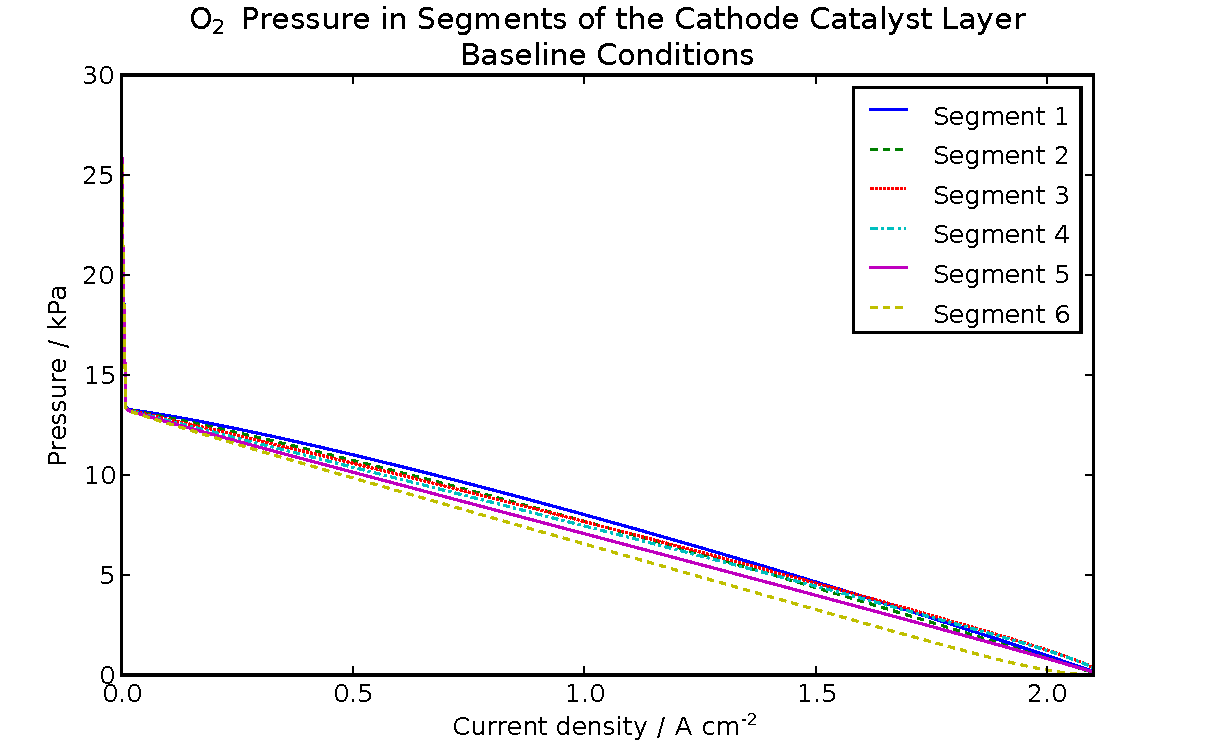
\includegraphics[width=\linewidth]{Results/Cell/Model/Segmented/CaCLO2Pressure}}
  \caption{Pressure of \s{O2} in the cathode catalyst layer of the segmented cell}
  \label{fig:SegmentO2Pressure}
\end{figure}

The upstream segments produce more electrical current due to the higher \n{O2} pressure and lower overpotentials, which are shown in \autoref{fig:SegmentOverpot}.  Although the efficiency is higher in the upstream segments, those segments produce more heat due to the higher current.  The rates of heat generation due to the \n{ORR} in the segments is shown in \autoref{fig:SegmentHeatGen}.  This causes the upstream segments to have higher temperature, as shown in \autoref{fig:SegmentTemperature}.  The higher temperature further reduces the overpotential in the upstream segments due to the activation energy.

\begin{figure}[htbp]
  \fbox{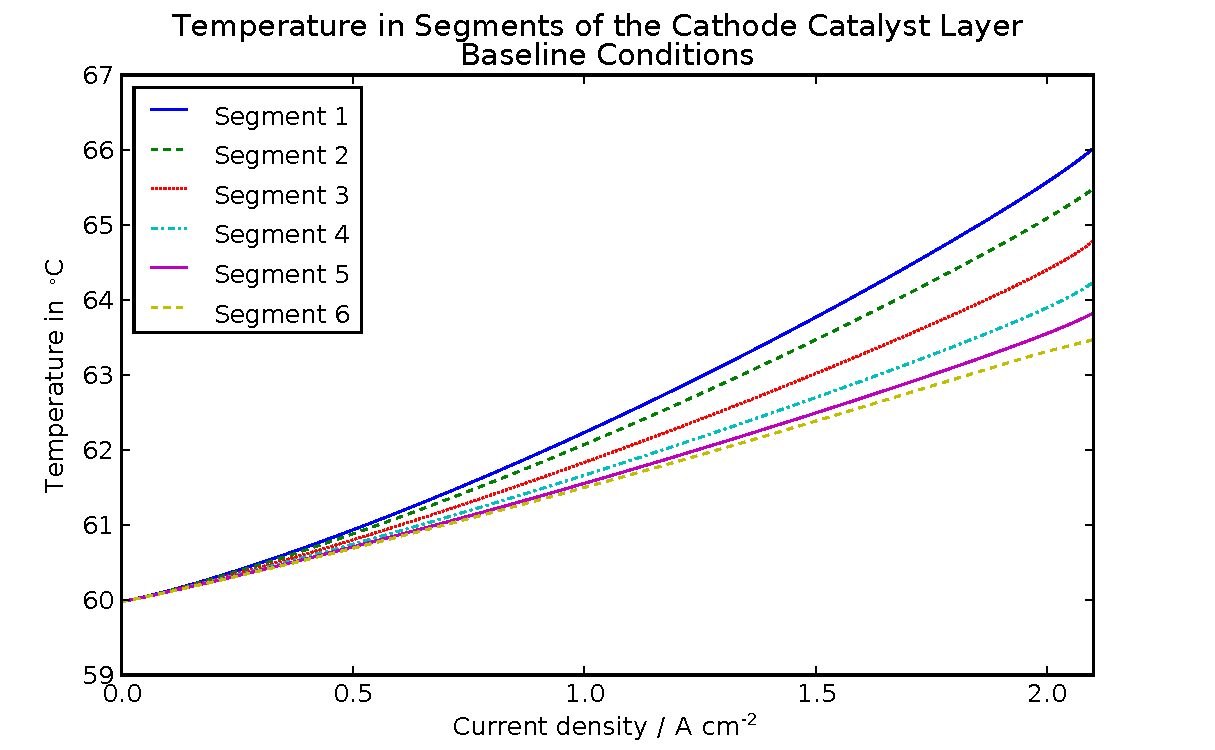
\includegraphics[width=\linewidth]{Results/Cell/Model/Segmented/CaCLTemperature}}
  \caption{Temperature in the cathode catalyst layer of the segmented cell}
  \label{fig:SegmentTemperature}
\end{figure}

\begin{figure}[htbp]
  \fbox{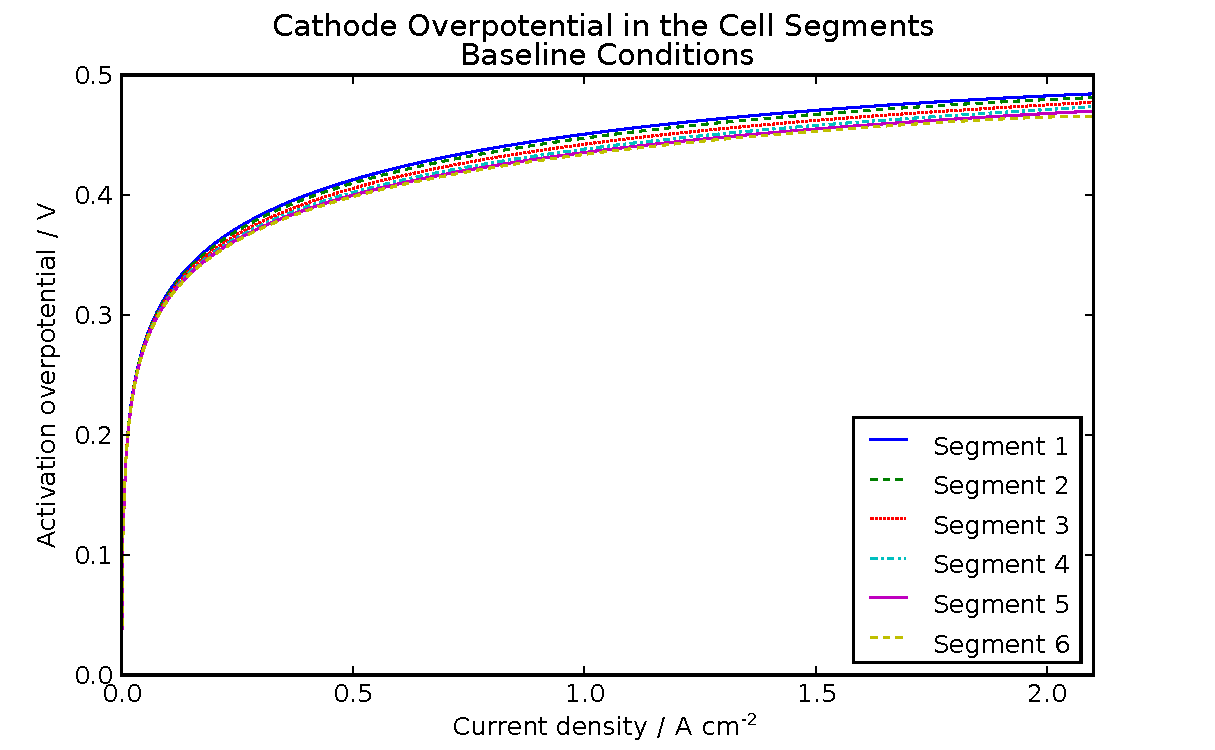
\includegraphics[width=\linewidth]{Results/Cell/Model/Segmented/CaOverpotential}}
  \caption{Overpotentials in the cathode of the cell segments}
  \label{fig:SegmentOverpot}
\end{figure}

\begin{figure}[htbp]
  \fbox{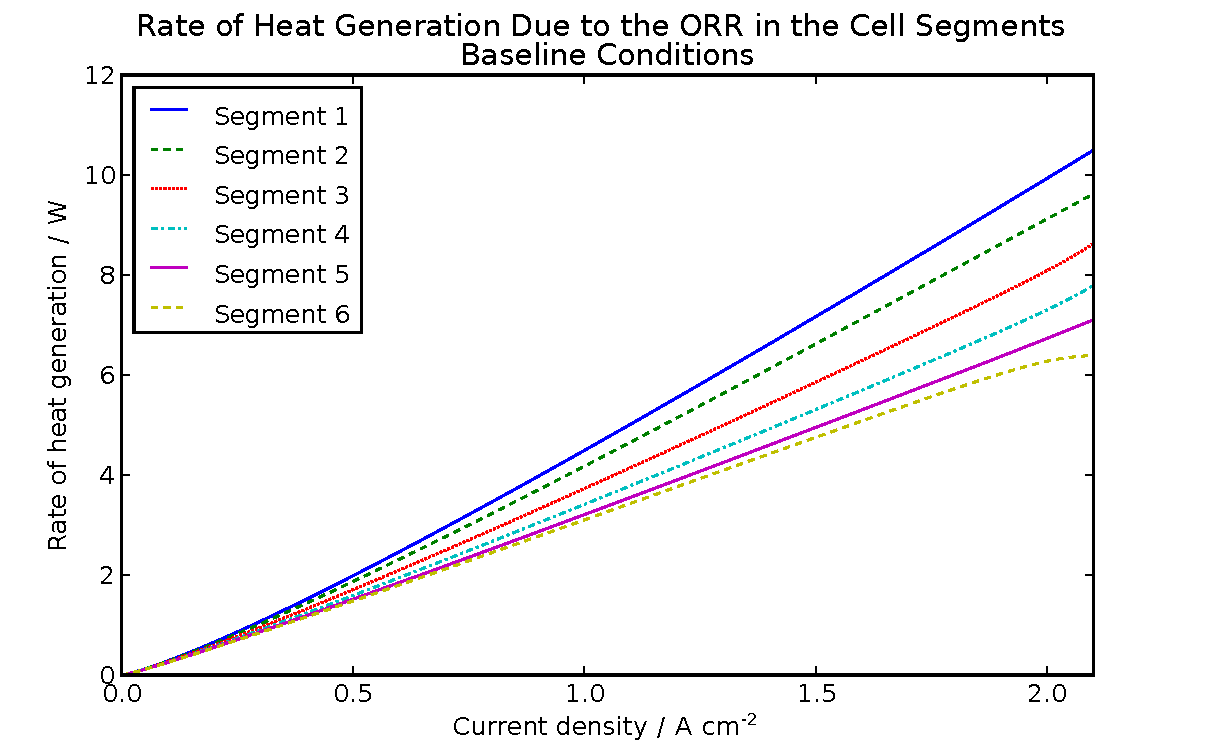
\includegraphics[width=\linewidth]{Results/Cell/Model/Segmented/CaHeatGen}}
  \caption[Rates of heat generation due to the ORR in the cell segments]{Rates of heat generation due to the \n{ORR} in the cell segments}
  \label{fig:SegmentHeatGen}
\end{figure}


\FloatBarrier % Flush the floats.
\section{Cyclical Load}
\label{sec:Cycle}

\subsection{Conditions}

This example demonstrates the dynamics of the cell model.  The ramping current load of the \modelica{TestStand} model (\autoref{fig:TestStandD}) is replaced with a sinusoidal current load as shown in \autoref{fig:TestStandCycleD}.  The amplitude is \SI{140}{mA/cm^2} and the offset is \SI{80}{mA/cm^2}, as shown in \autoref{fig:CycleLoad}.  To demonstrate the flexibility of the model, the minimum current density is negative (\SI{-60}{mA/cm^2}).  The frequency is \SI{0.3}{Hz}, and roughly three cycles are simulated.  The anode and cathode supplies are fixed at equivalent currents of 300 and \SI{400}{mA/cm^2}.  The electrolytic double layer models are included (not in the standard model).

\begin{figure}[htbp]
  \fbox{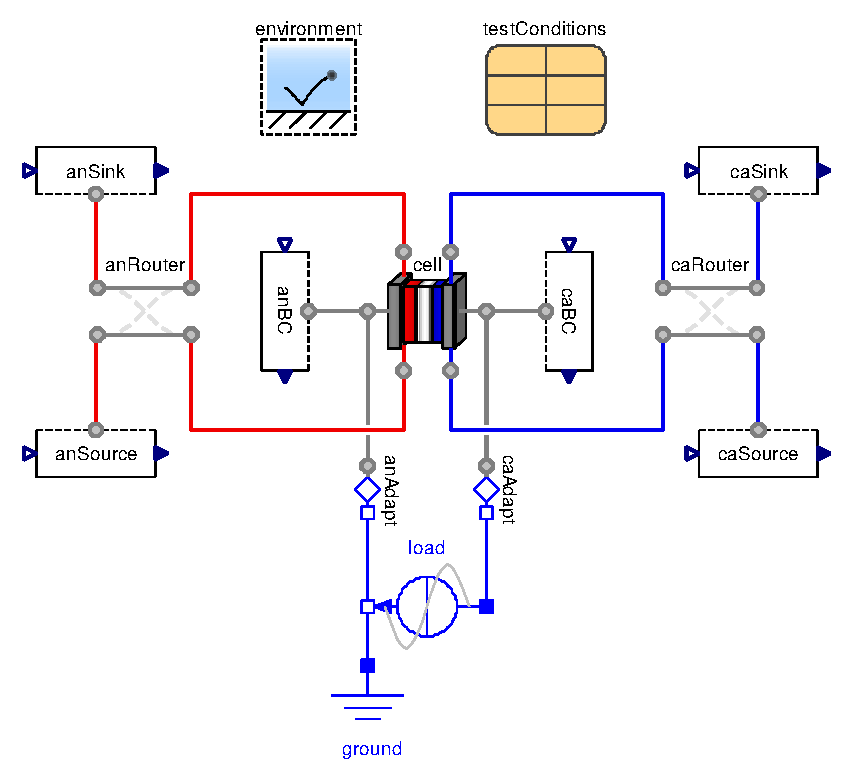
\includegraphics[width=\linewidth]{4-TestStandCycleD}}
  \caption{Model diagram for the test with a cyclical load}
  \label{fig:TestStandCycleD}
\end{figure}

\begin{figure}[htbp]
  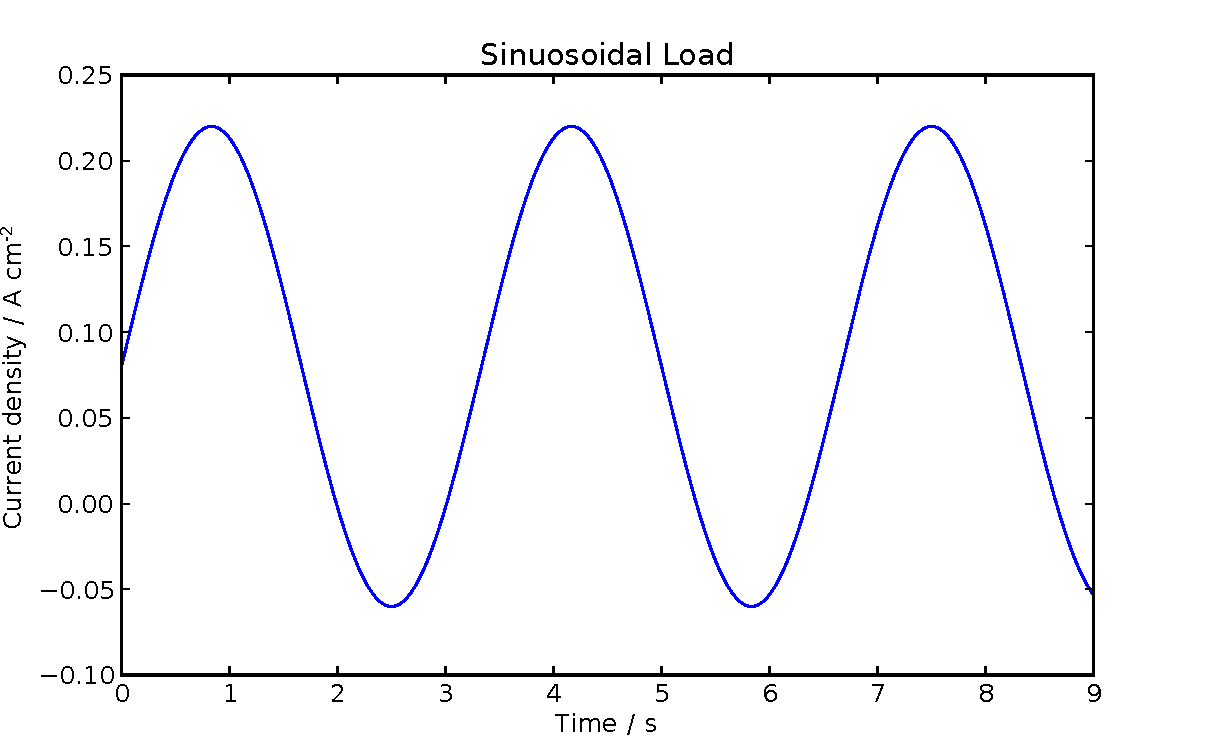
\includegraphics[width=\linewidth]{Results/Cell/Model/Cycle/Load}%
  \caption{Cyclical load applied to the cell (sinusoidal, reversing)}%
  \label{fig:CycleLoad}
\end{figure}

\subsection{Results and Discussion}

\begin{contextbox}
  Modeling and simulation statistics:
  \begin{itemize}
    \item Number of variables: 6942
    \item Number of time-varying variables: 2790
    \item Number of states: 57
    \item Sizes of the nonlinear systems of equations: None
    \item Sizes of the linear systems of equations: 1 set of 9, 1 set of 8, 1 set of 6, 2 sets of 5, 9 sets of 4, 20 sets of 3, 97 sets of 2
    \item Translation time: \SI{23}{s}
    \item Simulation time: \SI{4.03}{s}
  \end{itemize}
\end{contextbox}

As before, the model has no nonlinear systems of equations after translation.  This example requires approximately twice as long to simulate as the baseline polarization test.  

\autoref{fig:CyclePolarization} shows the current and voltage of the cell.  The voltage lags the current primarily due to the double layer capacitance.  There is a short settling period before a repeatable loop is established.  

\begin{figure}[htbp]
  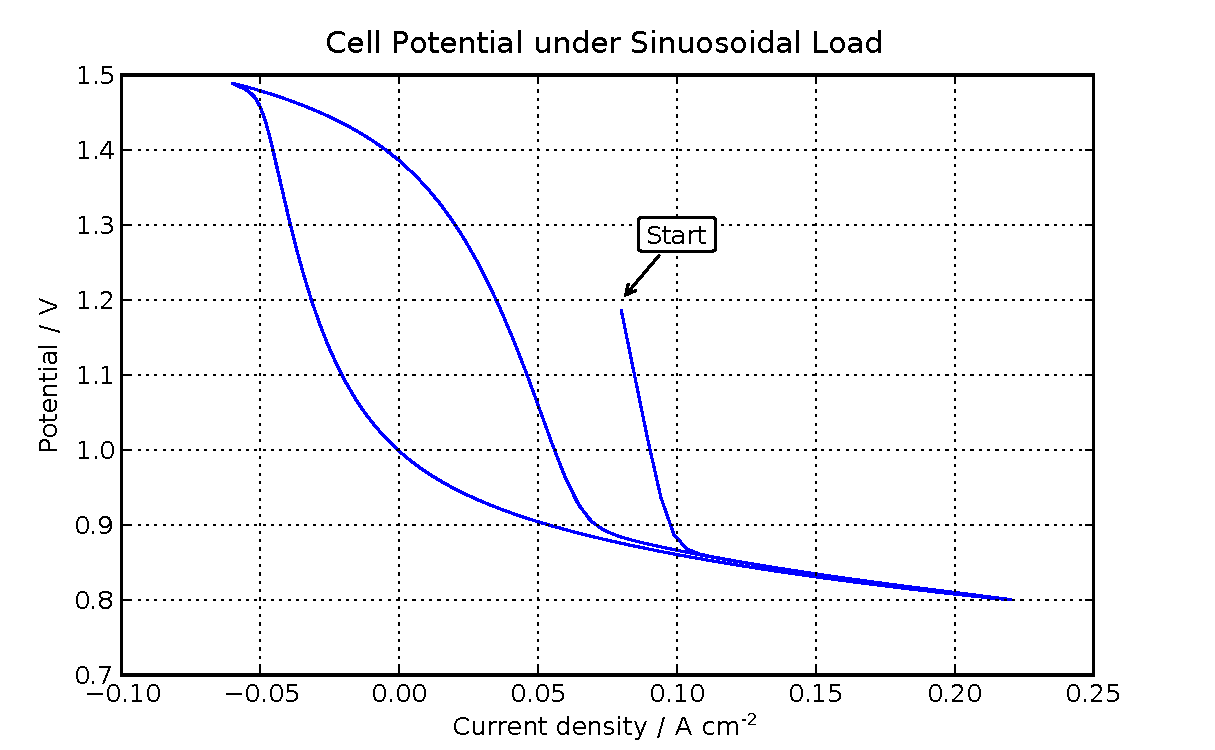
\includegraphics[width=\linewidth]{Results/Cell/Model/Cycle/Polarization}%
  \caption{Current and voltage under cyclical load}%
  \label{fig:CyclePolarization}
\end{figure}

\autoref{fig:CycleTemperature} shows the temperatures throughout the cell.  As before, the cathode catalyst layer reaches the highest temperature.  However, when the current reverses, the reaction is endothermic and the temperature of the cathode \n{GDL}, cathode catalyst layer, and \n{PEM} decrease.  

\begin{figure}[htbp]
  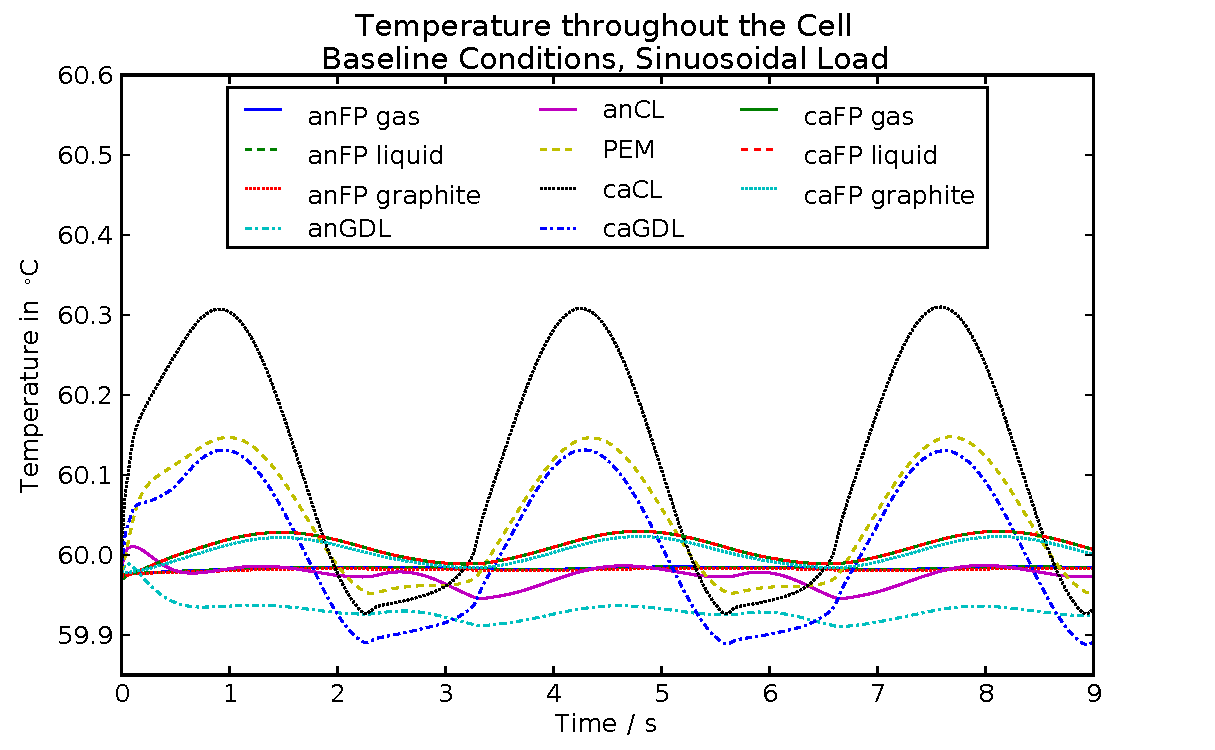
\includegraphics[width=\linewidth]{Results/Cell/Model/Cycle/Temperature}%
  \caption{Temperatures of throughout the cell under cyclical load}%
  \label{fig:CycleTemperature}
\end{figure}

\autoref{fig:CyclePressure} shows the pressure throughout the cell.  The pressures are highest in the catalyst layer at the peak rate of production of \n{H2} and \n{O2}.  The pressures are lowest at the peak rate of production of water, since the reactant gases must be drawn into the catalyst.  The production of water also increases the relative humidity of the gas and fills the pores of the cathode catalyst layer and \n{GDL}, as shown in Figures~\ref{fig:CycleHumidity} and \ref{fig:CyclePoreSaturation}.

\begin{figure}[htbp]
  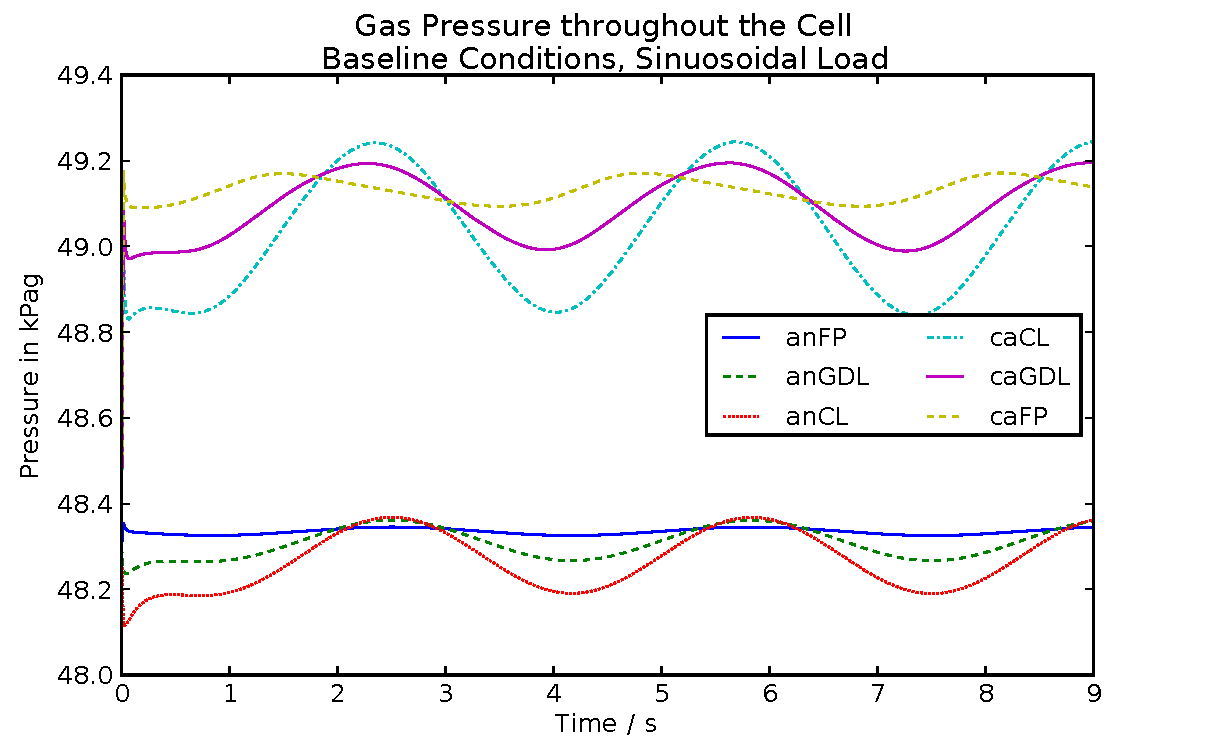
\includegraphics[width=\linewidth]{Results/Cell/Model/Cycle/PressureGas}%
  \caption{Gas pressure throughout the cell under cyclical load}%
  \label{fig:CyclePressure}
\end{figure}

\begin{figure}[htbp]
  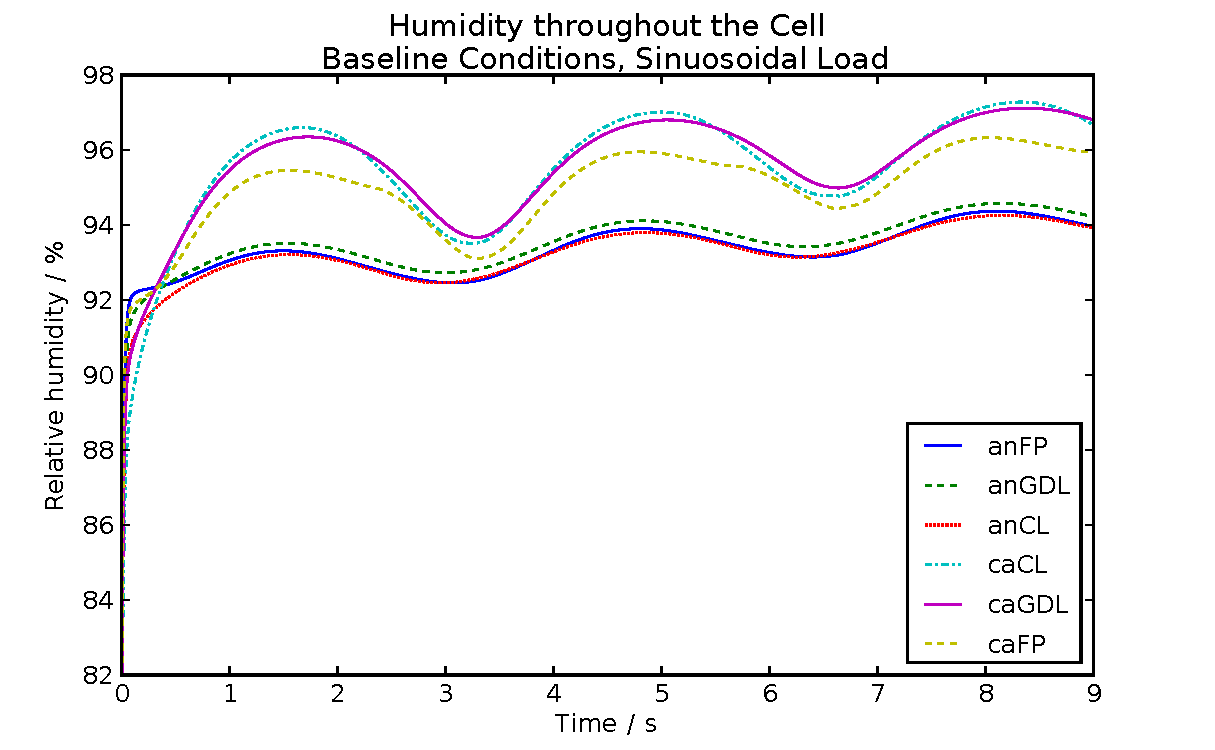
\includegraphics[width=\linewidth]{Results/Cell/Model/Cycle/Humidity}
  \caption{Relative humidity under cyclical load}%
  \label{fig:CycleHumidity}
\end{figure}

\begin{figure}[htbp]
  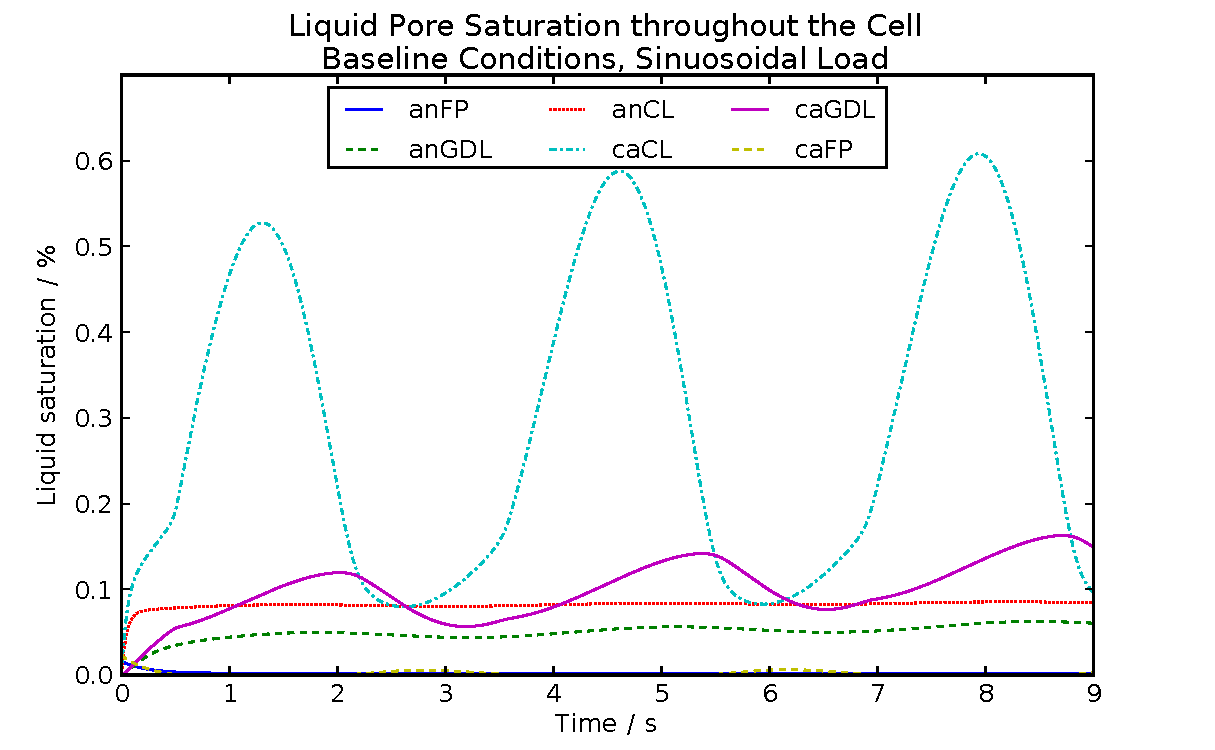
\includegraphics[width=\linewidth]{Results/Cell/Model/Cycle/PoreSaturation}%
  \caption{Liquid pore saturation under cyclical load}%
  \label{fig:CyclePoreSaturation}
\end{figure}

\autoref{fig:CycleHydration} shows the effect of the cyclical load on the hydration of the ionomer.  There is little net change in the hydration of the \n{MEA} since the rate of phase change between the ionomer and the liquid is slow relative to the frequency of the load.  However, when water is being produced, electro-osmotic drag causes the cathode side of the \n{MEA} to become more hydrated at the expense of the anode side.  When water is consumed, protons travel to the anode while dragging water and hydrating the anode side.  On average, the cathode side is more hydrated because the sinusoidal offset is positive---biased towards water production in the cathode.

\begin{figure}[htbp]
  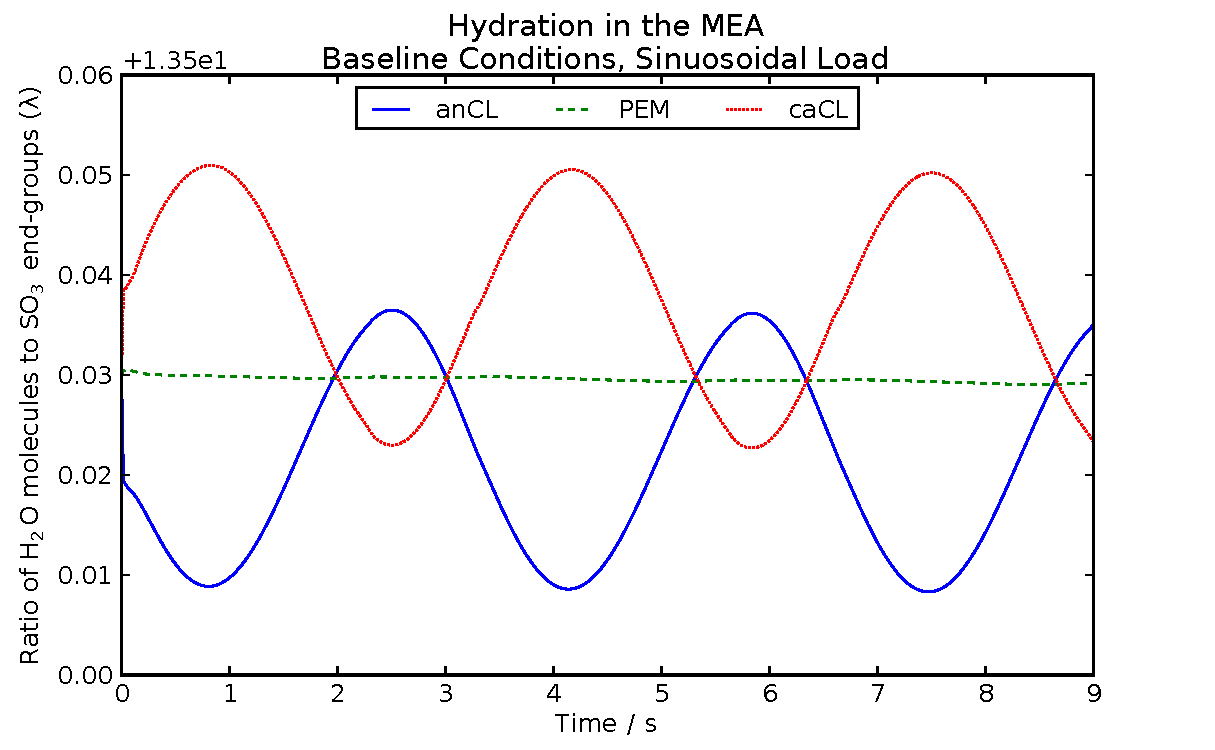
\includegraphics[width=\linewidth]{Results/Cell/Model/Cycle/Hydration}
  \caption{Hydration under cyclical load}%
  \label{fig:CycleHydration}
\end{figure}



\section{Summary}

This chapter provided examples of the fuel cell model.  Polarization tests were performed and compared to experimental results.  The qualitative trends are in basic agreement with the experimental results.  However, there are significant quantitative differences which may be due to hydrogen crossover and more complex behavior of liquid water in the experimental cell.  The differences could also be due to the large number of parameters in the model and the remaining uncertainty in their settings.  As demonstrated by the examples of simplified and segmented cell models, the modeling framework is reconfigurable.  As was shown under a cyclical load, the fuel cell model is also dynamic.

